\documentclass[a4paper, 11pt]{article}

\usepackage[export]{adjustbox}
\usepackage{wrapfig}
% \usepackage[french]{babel} error with tokens pckg.

\usepackage{tokens}

\usepackage[utf8]{inputenc}
\usepackage[T1]{fontenc}

\usepackage[margin=2cm]{geometry}

\usepackage{graphicx}
\usepackage{subcaption}
\usepackage{float}
\usepackage{color, colortbl, xcolor}
\usepackage{scalefnt}
\usepackage{lmodern}
\usepackage{titling}

\usepackage{amssymb,amsmath,amsthm}
\newtheorem{theorem}{Theorem}[section]
\newtheorem{corollary}{Corollary}[theorem]
\newtheorem{lemma}[theorem]{Lemma}
\renewcommand\qedsymbol{$\blacksquare$}
\renewcommand{\proofname}{\rm\bf{Preuve}}

\usepackage[hidelinks]{hyperref}

\usepackage{tikz}
\usetikzlibrary{shapes.geometric}
\usetikzlibrary{arrows}
\usetikzlibrary{shapes.arrows}
\usetikzlibrary{decorations.markings}

\usepackage[simplified]{pgf-umlcd}
\usepackage{listings}

\usepackage{rotating}
\usepackage{pgfgantt}
\usepackage{scalefnt}

\usepackage[toc,page]{appendix}
\renewcommand{\appendixtocname}{Annexes} 


\title{Programmation Récursive Primitive sur les Ensembles Purs}
\author{Alexandre Clément}
\date{1 Septembre 2019}

\graphicspath{ {images/} }


\newcommand{\HRule}{\rule{\linewidth}{0.5mm}}

\renewcommand{\maketitle}{
    \begin{titlepage}
        \begin{figure}[h]
            \begin{subfigure}{0.5\textwidth}
                \includegraphics[height=0.2\linewidth, left]{unice.png}
            \end{subfigure}
            \begin{subfigure}{0.5\textwidth}
                \includegraphics[height=0.2\linewidth, right]{polytech.png}
            \end{subfigure}
        \end{figure}
        \vfill
        \begin{center}
            \textsc{\LARGE Rapport final}
            \HRule \\ [0.4 cm]
            \textsc{\huge \bfseries \thetitle}
            \HRule \\ [0.4 cm]
            {\large Laboratoire i3s \\ Sophia Antipolis, Alpes-Maritimes, France \\ \thedate}
        \end{center}
        \vfill
        \begin{minipage}[t]{0.60\textwidth}
            \begin{flushleft} 
                \large\emph{Auteur :} \theauthor \\
                \large\emph{Formation :} Science Informatique \\
                \large\emph{Parcours :} Architecture Logicielle
            \end{flushleft}
          \end{minipage}
          \begin{minipage}[t]{0.42\textwidth}
            \begin{flushleft}
                \large\emph{Encadrant :} M.~Christophe \textsc{Papazian} \\
                \large\emph{Co-encadrant :} M.~Grégory \textsc{Lafitte} \\
                \emph{Tuteur :} M.~Igor \textsc{Litovsky} \\ 
            \end{flushleft}
        \end{minipage}
    \end{titlepage}
}

\renewcommand{\contentsname}{Table des matières}

\begin{document}

\maketitle

\newgeometry{top=1.7cm, bottom=1.7cm}  

\tableofcontents

\restoregeometry

\newpage

\section*{Remerciements}

Je tiens à remercier toutes les personnes qui ont contribué 
au succès de mon stage et qui m'ont aidé lors de la rédaction de ce rapport.

Je tiens tout d'abord à remercier vivement mon encadrant de stage,
M. Christophe Papazian qui m'a encadré et guidé durant ce stage.

Je remercie également M. Igor Litovsky pour avoir accepté d'être 
mon tuteur enseignant pour ce stage.

Enfin, je remercie M. Grégory Lafitte qui a apporté son aide au cours de ce stage.

\newpage

\section{Introduction}

En calculabilité, les fonctions récursives primitives sont une classe de 
fonctions définies à partir de la composition et d'une récursion primitive.
Ce concept a d'abord été imaginé par Richard Dedekind en 1888 avant d'être 
formalisé par Rózsa Péter en 1934.
Les fonctions primitives ont d'abord été définies sur les entiers naturels à
partir des axiomes de Peano. Les fonctions basiques étaient données à partir de
ces fonctions élémentaires atomiques:
\begin{enumerate}
    \item \textbf{Fonction constante}: la fonction constante notée E d'arité 0 est 
    récursive primitive.
    \item \textbf{Fonction successeur}: la fonction d'arité 1 qui renvoie le 
    successeur est récursive primitive. Il s'agit de $S: k \mapsto k + 1$.
    \item \textbf{Projecteur}: Pour tout $n > 1$ et pour tout i avec 
    $1 \leq i \leq n$, la fonction d'arité n $P_i^n$, qui renvoie le $i^{ieme}$ 
    argument, est récursive primitive.
    Elle se note: $P_i^n: p_1, p_2, \dots, p_{i-1}, p_i, p_{i+1}, \dots, p_n \mapsto p_i$.
\end{enumerate}

Les fonctions primitives récursives plus complexes peuvent être obtenues en 
appliquant les opérations données par ces opérateurs de construction élémentaires:

\begin{enumerate}
    \setcounter{enumi}{3}
    \item \textbf{Composition}: Étant donné une fonction primitive récursive 
    d'arité $k$ et $k$ fonctions primitives récursives $g_1, ..., g_k$ d'arité
    $m$, la composition de $f$ par $g_1, ..., g_k$ est la fonction $h$ telle que
    $h(x_1, ..., x_m) = f(g_1(x_1, ..., x_m), ..., g_k(x_1, ..., x_m))$.
    La fonction $h$ est récursive primitive.

    \item \textbf{Récursion}: Étant donné une fonction
    primitive récursive d'arité k, et g une fonction primitive récursive d'arité $k+2$,
    la fonction $h$ d'arité $k+1$ est la récursion primitive \label{recusion primitive}
    de $f$ et $g$ i.e la fonction $h$ est primitive récursive quand
    \begin{itemize}
        \item $h(0, x_1, ..., x_k) = f(x_1, ..., x_k)$ et
        \item $h(S(y), x_1, ..., x_k) = g(y, h(y, x_1, ..., x_k), x_1, ..., x_k)$.
    \end{itemize}
\end{enumerate} 

Une grande partie des fonctions de la théorie des nombres sont récursives 
primitives. Par exemple, on peut définir l'addition, la division, 
la factorielle et toutes les fonctions mathématiques usuelles

\subsection{Avantages et limitations}

Par construction de la récursion primitive, on est assuré que tous les
programmes se terminent. En revanche, cela nous restreint quant aux fonctions
pouvant être calculées. On peut citer l'exemple de la fonction d'Ackermann-Peter qui 
est définie récursivement, mais qui n'est pas récursive primitive.
Toutefois, toute fonction dont la complexité est bornée par une fonction récursive
primitive est elle même récursive primitive. Ainsi, comme la classe des fonctions 
récursives primitives contient les fonctions arithmétiques usuelles 
(polynômes, exponentielles, tours d'exponentielles ...), elle contient aussi toutes 
les classes de complexité usuelles, et en particulier P, NP, EXP et PSPACE.

\subsection{Généralisation aux ensembles}

Dans ce stage, nous allons nous intéresser aux fonctions primitives récursives
appliquées aux ensembles purs de la théorie des ensembles de Zermelo-Fraenkel (ZF).
Les fonctions primitives de base issues des axiomes de Peano sont ainsi
remplacées par les fonctions primitives récursives issues des axiomes de ZF.
La fonction projecteur et la composition sont conservées. La récursion primitive
va devoir être modifiée pour correspondre aux ensembles \cite{jensen1971primitive}. 

\def\unionplus{\ensuremath{\kern-0.4pt\adjustbox{lap=0.5\width}{$\bigcup$}\adjustbox{scale=2,lap=-0.5\width, raise=-0.35em}{$\cdot$}}}
\def\ifthenelse{\ensuremath{\kern-0.4pt\adjustbox{lap=0.5\width}{$?$}\adjustbox{scale=1,lap=-0.1\width}{$\in$}}}

\begin{enumerate}
    \item \textbf{L'ensemble vide}: la fonction constante E d'arité 0 
    notée $E: () \mapsto \emptyset$.
    \item \textbf{Fonction union}: la fonction d'arité 2 qui a $(x, y)$, renvoie 
    l'union de $x$ et de $\{y\}$. Il s'agit de $x \ \unionplus \ y = x \cup \{y\}$.
    \item \textbf{Fonction d'appartenance}: la fonction d'arité 4 qui a $(x, y, u, v)$
    renvoie $x$ si $u \in v$, y sinon. Elle est notée $if(x, y, u, v) \mapsto x$
    si $u \in v$ sinon $y$.
    \item \textbf{Récursion}: Étant donné une fonction
    primitive récursive d'arité $k+2$, la fonction $h$ d'arité $k+1$ est la 
    récursion primitive de $f$ i.e la fonction $h$ est récursive primitive tel que
    \[h(z, x_1, ..., x_k) = f(\bigcup_{u \in z} h(u, x_1, ..., x_k), z, x_1, ..., x_k)\].
    Cette définition de la fonction de récursion est limitée car le nombre d'appels récursifs est
    limité par le rang de l'entrée (voir \ref{rang} pour la définition du rang d'un ensemble).
    Cela a deux conséquences : 
    \begin{itemize}
        \item tous les calculs utilisent des ressources finies sur les entrées héréditairement finies;
        \item sur les ensembles de rang infini, nos calculs sont bornés par les rangs en entrée, 
        ce qui explique que le calcul termine toujours, même si on utilise alors une mémoire infinie 
        et une capacité infinie de parallélisation des calculs : 
        comme nos ensembles sont bien fondés, tous les chemins descendants dans l’ensemble sont finis.
    \end{itemize}

\end{enumerate}

\subsubsection{Classe d'ensemble}

Comme nous manipulons des ensembles dans notre modèle, on utilise le terme
de "classe" pour référer à une collection d'objets de notre modèle, cette collection
pouvant ne pas faire partie du modèle. \cite{devlin_1981}
On peut alors définir toutes sortes de classes:

\begin{itemize}
    \item \textbf{singleton}: les singletons sont les ensembles ne contenant qu'un seul élément. 
    \item \textbf{paire}: les paires sont les ensembles contenant exactement 2 éléments.
    \item \textbf{couple}: les couples sont les ensembles contenant exactement 2 éléments dans un ordre déterminé.
    Pour représenter un couple sous forme d'ensemble, on utilise la représentation de 
    Kuratowski \cite{kuratowski1921notion} dans laquelle le couple $(x,y) = \{\{x\}, \{x, y\}\}$.
    \item \textbf{tuple}: à partir des couples, on peut construire des tuples de tailles quelconques.
    On définie les tuples de manière récursive de la façon suivante: 
    $(e_1, e_2, \dots, e_n) = (e_1, (e_2, \dots, e_n))$. On transforme ainsi le tuple
    de taille n $(e_1, e_2, \dots, e_n)$ en un couple contenant l'élément $e_1$ et le
    tuple de taille $n-1$ $(e_2, \dots, e_n)$.
    \item \textbf{liste}: de manière analogue aux tuples, on peut définir les listes.
    On commence par définir la liste vide $[] = \emptyset$. Puis la liste contenant 
    uniquement l'élément $x$ comme étant le couple contenant $x$ et la liste vide:
     $[x] = (x, []) = (x, \emptyset)$.
    La liste $[x, y]$ se simpifie donc en $(x, [y]) = (x, (y, [])) = (x, (y, \emptyset))$.
    Dans le cas général, la liste $[x_1, x_2, \dots, x_n] = (x_1, [x_2, \dots, x_n])$.
    \item \textbf{relation}: les relations sont les ensembles de la forme 
    $\{(x, y), x \in X, y \in Y\}$ qu'on note plus généralement $xRy \iff (x, y) \in R$.
    \item \textbf{fonction}: $R$ est une fonction si $\forall x, y, z, xRy \wedge xRz \implies y = z$.
\end{itemize}

\subsubsection{Nombre ordinal}

Un nombre ordinal est un ensemble qui vérifie les deux propriétés suivantes:
\begin{enumerate}
    \item La relation d'appartenance $\in$ est un bon ordre strict, c'est à dire:
    \begin{itemize}
        \item \textbf{ordre strict}: $\in$ est antiréflexive et transitive
        \item \textbf{bon ordre}: toute partie non vide d'un ensemble $\alpha$ a un plus petit élément
    \end{itemize}

    \item Cet ensemble est \textbf{transitif}, ce qui s'écrit:
    \[\forall x \in \alpha, x \subset \alpha\]
\end{enumerate}

En appliquant la définition précédente, les entiers naturels peuvent être construits
de la façon suivante:
\[0 = \emptyset\]
\[n + 1 = n \cup \{n\}\]

Un entiers positif est ainsi identifié à l'aide de ses prédécesseurs:
\begin{itemize}
    \item $0 = \{\} = \emptyset$
    \item $1 = \{0\} = \{\{\}\}$
    \item $2 = \{0, 1\} = \{\{\}, \{\{\}\}\}$
    \item $3 = \{0, 1, 2\} = \{\{\}, \{\{\}\}, \{\{\}, \{\{\}\}\}\}$
    \item $4 = \{0, 1, 2, 3\} = \{\{\}, \{\{\}\}, \{\{\}, \{\{\}\}\}, \{\{\}, \{\{\}\}, \{\{\}, \{\{\}\}\}\}\}$
    \item etc.
\end{itemize}

Tous ces ordinaux qui correspondent aux entiers naturels sont dits héréditairement finis,
cela signifie que tous ces
ensembles sont finis et leurs éléments sont également héréditairement finis.

\subsubsection{Ordinal limite}

Un ordinal limite est un ordinal qui n'a pas de prédécesseur.
Le premier ordinal limite est noté $\omega$.
Il correspond à l'ensemble des entiers naturels $\mathbb N = \{0, 1, 2, 3, \dots\}$.
Remarquons que $\omega$ est également
le premier ordinal transfini (voir \ref{transfinie}).
L'ordinal qui suit est $\omega + 1 = \omega \cup \{\omega\}$. L'ordinal limite suivant
est $\omega + \omega = \omega \times 2$, suivi par $\omega \times n$ pour tout entier naturel $n$.
\'{A} partir de la réunion de tous les $\omega \times n$, on obtient $\omega \times \omega = \omega^2$.
Ce procédé peut être itéré pour produire 
$\omega^3, \omega^4, \dots, \omega^\omega, \omega^{\omega^\omega}, \dots, 
\epsilon_0 = \omega^{\omega^{\omega^{.^{.^{.}}}}}, \dots$.

\subsubsection{Propriétés des ensembles}

\begin{itemize}
    \item \textbf{Clôture transitive} \label{cloture transitive}: La clôture transitive d'un ensemble
    est le plus petit ensemble transitif contenant l'ensemble de départ.
    \item \textbf{Descendants} \label{descendants}: Les descendants d'un ensemble sont les éléments de
    sa clôture transitive.
    \item \textbf{Rang}: \label{rang} On définit le rang d'un ensemble comme étant sa profondeur, 
    on a ainsi:
    \begin{itemize}
        \item $rang(\emptyset) = 0$ et
        \item $rang(x) = \underset{u \in x}{sup}(rang(u) + 1)$
    \end{itemize}
    Remarquons que dans notre modèle, nos ensembles sont bien-fondés, ce qui signifie
    qu'ils ne peuvent pas se contenir eux-mêmes.
    \item \textbf{Cardinalité}: On définit la cardinalité d'un ensemble fini comme 
    étant le nombre d'éléments qu'il contient. Plus généralement, le cardinal d'un
    ensemble est le plus petit ordinal équipotent à celui-ci.
    Remarquons que comme l'opérateur de récursion est appliqué récursivement sur 
    les éléments d'un ensemble, on peut facilement calculer le rang de celui-ci.
    En revanche, on ne peut généralement pas déterminer sa cardinalité.
    \item \textbf{Héréditairement fini}: un ensemble est héréditairement fini s'il
    contient un nombre fini d'éléments et si tous ses éléments sont héréditairement finis.
    \item \textbf{Nombre transfini} \label{transfinie}: un nombre transfini est un ordinal qui n'est pas fini.
    Le plus petit nombre transfini est $\omega$.
\end{itemize}

\subsection{Représentation des ensembles}

\def\bigdot{\ensuremath{\adjustbox{scale=2,raise=-0.35em}{$\cdot$}}}

Nous allons, dans cette partie, définir une représentation sous forme d'arbre pour les
ensembles. Cela nous permettra en particulier de mieux comprendre le comportement
de certains programmes. Un noeud de l'arbre représente un ensemble et ses enfants
représentent les éléments de cet ensemble. Les feuilles de cet arbre sont des ensembles
sans éléments, par conséquent, les feuilles représentent l'ensemble vide.

\begin{itemize}
    \item L'ensemble $1 = \{0\} = \{\{\}\}$ peut être représenté par
    \begin{figure}[!ht]
        \fboxsep=5mm
        \centering{
            \hfill
            \fbox{
            \begin{tikzpicture}[
                sibling distance=5cm, 
                level 2/.style={sibling distance =2cm},
                triangle/.style={isosceles triangle,draw,shape border rotate=90, dashed, minimum height=10mm, minimum width=15mm, inner sep=0},
                ]
                \node [] {$\bigdot$}
                    child { node[] {$\bigdot$} };
            \end{tikzpicture}
        }
        \hfill
        \fbox{
            \begin{tikzpicture}[
                sibling distance=5cm, 
                level 2/.style={sibling distance =2cm},
                triangle/.style={isosceles triangle,draw,shape border rotate=90, dashed, minimum height=10mm, minimum width=15mm, inner sep=0},
                ]
                \node [] {$\bigdot$}
                    child { node[] {$0$} };
            \end{tikzpicture}
        }
        \hfill
        }
    \end{figure}
    \item De manière plus générale, l'ensemble singleton $\{x\}$ peut être représenté par
    \begin{figure}[!ht]
        \fboxsep=5mm
        \centering\fbox{
            \begin{tikzpicture}[
                sibling distance=5cm, 
                level 2/.style={sibling distance =2cm},
                triangle/.style={isosceles triangle,draw,shape border rotate=90, dashed, minimum height=10mm, minimum width=15mm, inner sep=0},
                ]
                \node [] {$\bigdot$}
                    child { node[] {$x$} };
            \end{tikzpicture}
        }
    \end{figure}
    \item L'ensemble $2 = \{0, 1\} = \{\{\}, \{\{\}\}\}$ peut être représenté par
    \begin{figure}[H]
        \fboxsep=5mm
        \centering{
            \hfill
            \fbox{
            \begin{tikzpicture}[
                sibling distance=5cm, 
                level 2/.style={sibling distance =2cm},
                triangle/.style={isosceles triangle,draw,shape border rotate=90, dashed, minimum height=10mm, minimum width=15mm, inner sep=0},
                ]
                \node [] {$\bigdot$}
                    child { node[] {$\bigdot$} }
                    child { node[] {$\bigdot$} child { node[] {$\bigdot$} } 
                };
            \end{tikzpicture}}
            \hfill
            \fbox{
            \begin{tikzpicture}[
                sibling distance=5cm, 
                level 2/.style={sibling distance =2cm},
                triangle/.style={isosceles triangle,draw,shape border rotate=90, dashed, minimum height=10mm, minimum width=15mm, inner sep=0},
                ]
                \node [] {$\bigdot$}
                    child { node[] {$0$} }
                    child { node[] {$\bigdot$} child { node[] {$0$} } 
                };
            \end{tikzpicture}}
            \hfill
            \vspace{0.5cm}
            \fbox{
            \begin{tikzpicture}[
                sibling distance=5cm, 
                level 2/.style={sibling distance =2cm},
                triangle/.style={isosceles triangle,draw,shape border rotate=90, dashed, minimum height=10mm, minimum width=15mm, inner sep=0},
                ]
                \node [] {$\bigdot$}
                    child { node[] {$0$} }
                    child { node[] {$1$} 
                };
            \end{tikzpicture}}
        }
    \end{figure}
    \item De manière plus générale, l'ensemble paire $\{x, y\}$ peut être représenté par
    \begin{figure}[!ht]
        \fboxsep=5mm
        \centering\fbox{
            \begin{tikzpicture}[
                sibling distance=5cm, 
                level 2/.style={sibling distance =2cm},
                triangle/.style={isosceles triangle,draw,shape border rotate=90, dashed, minimum height=10mm, minimum width=15mm, inner sep=0},
                ]
                \node [] {$\bigdot$}
                    child { node[] {$x$} }
                    child { node[] {$y$} };
            \end{tikzpicture}
        }
    \end{figure}
    \item l'ensemble représentant l'opération $x \ \unionplus \ y$ peut être représenté par
    \begin{figure}[!ht]
        \fboxsep=5mm
        \centering\fbox{
            \begin{tikzpicture}[
                sibling distance=5cm, 
                level 2/.style={sibling distance =2cm},
                subset/.style={draw,dashed,shape border uses incircle,
                isosceles triangle,isosceles triangle apex angle=110,
                shape border rotate=-55,yshift=0.3cm, xshift=1.5cm,
                minimum height=0.9cm},
                ]
                \node [] {$\bigdot$}
                    child { node[subset] {$x$}  edge from parent[draw=none] }
                    child { node[] {$y$} };
            \end{tikzpicture}
        }
    \end{figure}

    $x$ est sous-arbre de l'ensemble
    $x \ \unionplus \ y = x \cup \{y\}$ car tous les éléments de $x$ appartiennent 
    à l'ensemble $x \ \unionplus \ y$.
\end{itemize}

\newpage

\subsection{Description des jetons \label{jetons}}

Les fonctions récursives primitives peuvent être représentées efficacement 
par des programmes écrits sous la forme de suites de jetons représentant les 
instructions atomiques de ce modèle de calcul.

On énumère ici les jetons de notre modèle de calcul, par exemple, le jeton
\progS{E} est le programme qui représente la fonction d'arité $0$ notée
$E: () \mapsto \emptyset$.

\subsubsection{Fonctions initiales}

\begin{enumerate}
\item Le jeton correspondant à la \textbf{Fonction constante} E se note 

\progS{E} $[f_0]$: $()\mapsto \emptyset$.
\item Pour des raisons pratiques, notre modèle doit comporter un jeton identité

\progS{I} $[f_1]$: $(x)\mapsto x$.
\item Le jeton correspondant à la \textbf{Fonction successeur} se note \progS{+} $[f_2]$: $(x,y)\mapsto x\cup\{y\}$.
\item On ajoute également un jeton permettant de vérifier l'appartenance d'un élément à un autre ensemble.

\progS{?} $[f_4]$: $(x,y,u,v)\mapsto \mbox{si }u\in v\mbox{ alors }x\mbox{ sinon }y$

\end{enumerate}

\subsubsection{Projecteurs}

Le \textbf{Projecteur} est représenter par les deux jetons suivants.

\begin{enumerate}
    \setcounter{enumi}{4}
    \item \progS{<} $[f_n \rightarrow f_{n+1}]$: \progS{<!f}$(x,\bar{y})\mapsto \progS{!f}(\bar{y})$
    \item \progS{>} $[f_n \rightarrow f_{n+1}]$: \progS{>!f}$(\bar{y},x)\mapsto \progS{!f}(\bar{y})$
\end{enumerate}

\paragraph*{Exemple: } \begin{itemize}
    \item \progS{<I}: $(a, b) \mapsto b$
    \item \progS{<>I}: $(a, b, c) \mapsto b$
    \item \progS{<<>I}: $(a, b, c, d) \mapsto c$
    \item \progS{>>>I}: $(a, b, c, d) \mapsto a$
\end{itemize}

\newcommand{\projecteur}[2]{\mbox{\scriptsize\bfseries $\Pi^#1_#2$}}
% \def\projecteur#1#2{mbox{\scriptsize\bfseries $\Pi^#1_#2$}}
\def\proj{\projecteur{i}{n}}

Plus généralement, on peut construire le programme projecteur qui pour n arguments renvoie le $i^{ieme}$. \\
\progS{'\proj} : $(a_1, a_2, ... a_i, ..., a_n) \mapsto a_i$ = $\underbrace{\progS{<!\dots<}}_{i-1} \underbrace{\progS{>!\dots>}}_{n-i-1}$ \progS{I}. 

\subsubsection{Opérateurs}

\def\gone{\mbox{\scriptsize\bfseries $g_1$}}
\def\gtwo{\mbox{\scriptsize\bfseries $g_2$}}
\def\gdots{\mbox{\scriptsize\bfseries $\dots$}}
\def\gn{\mbox{\scriptsize\bfseries $g_n$}}

\begin{enumerate}
    \setcounter{enumi}{6}
    \item L'opérateur de \textbf{Composition} est représenter par le jeton suivant.
    
    \progS{o} $[f_{n+1}, f_p\times(n+1) \rightarrow f_{p}]$ 

    \progS{o!f!\gone!\gtwo}\dots\progS{!\gn} : $\displaystyle(\bar{x}) \mapsto \progS{!f}\left( \progS{!\gone} (\bar{x}), \progS{!\gtwo} (\bar{x}), \dots, \progS{!\gn} (\bar{x})\right) $

    \item L'opérateur de \textbf{Récursion} est représenter par le jeton suivant.
    
    \progS{R} $[f_{n+2} \rightarrow f_{n+1}]$ 

    \progS{R!f} : $\displaystyle(x,\bar{y}) \mapsto \progS{!f}\left(\bigcup_{z\in x} \progS{R!f}(z,\bar{y}), x, \bar{y}\right) $

\end{enumerate}

\subsubsection{Exemples}

\def\tc{\mbox{\scriptsize\bfseries TC}}

\begin{enumerate}
    \item On s'intéresse au programme d'arité 1 \progS{o+<EI}:
    \begin{align*}
        \progS{o+<EI}(\emptyset) & = \progS{+}(\progS{<E}(\emptyset), \progS{I}(\emptyset)) \\
        & = \progS{+}(\progS{E}(), \emptyset) \\
        & = \progS{+}(\emptyset, \emptyset) \\
        & = \emptyset \cup 1 \\
        & = 1 \\
        \progS{o+<EI}(1) & = \progS{+}(\progS{<E}(1), \progS{I}(1)) \\
        & = \progS{+}(\progS{E}(), 1) \\
        & = \progS{+}(\emptyset, 1) \\
        & = \emptyset \cup \{1\} \\
        & = \{1\} \\
        \progS{o+<EI}(2) & = \progS{+}(\progS{<E}(2), \progS{I}(2)) \\
        & = \progS{+}(\progS{E}(), 2) \\
        & = \progS{+}(\emptyset, 2) \\
        & = \emptyset \cup \{2\} \\
        & = \{2\}
    \end{align*}
    On déduit que \progS{o+>EI}: $z \mapsto \{z\}$

    On s'intéresse au programme d'arité 1 \progS{R+}: 
    \begin{align*}
        \progS{R+}(\emptyset) & = \progS{+}(\bigcup_{u \in \emptyset} \progS{R+}(u), \emptyset) \\
        & = 1 \\
        \progS{R+}(1) & = \progS{+}(\bigcup_{u \in 1}  \progS{R+}(u), 1) \\
        & = \progS{+}( \progS{R+}(\emptyset), 1) \\
        & = \progS{+}(1, 1) \\
        & = 2 \\
        \progS{R+}(\{1\}) & = \progS{+}(\bigcup_{u \in \{1\}}  \progS{R+}(u), \{1\}) \\
        & = \progS{+}( \progS{R+}(1), \{1\}) \\
        & = \progS{+}(2, \{1\}) \\
        & = \{\emptyset, 1, \{1\}\} \\
    \end{align*}
    Pour chaque récursion, le programme \progS{R+} ajoute l'élément $z$ à l'union des
    appels du programme \progS{R+} sur les éléments de $z$. Ainsi, on en déduit que le
    \progS{R+} construit récursivement un ensemble contenant tous les éléments
    de $z$ et de ses descendants. Cette fonction permet donc de calculer la clôture
    transitive d'un ensemble (voir \ref{cloture transitive}). 

    \progS{R+}: $(x)\mapsto \progS{'\tc}(\{x\})$ où 
    \progS{'\tc} est la clôture transitive.
\end{enumerate}

\subsubsection{Variantes}

Certains des jetons définis peuvent être dérivé sous différentes formes.
On peut par exemple nous intéresser au cas du jeton \progS{?} qui peut être
transformé sous forme d'opérateur tel que 

\progS{:!f!g} : $\displaystyle(\bar{x}, u, v) \mapsto \progS{!f}(\bar{x}, u, v) $ si $u \in v$ sinon $\progS{!g}(\bar{x}, u, v)$


\section{Problématiques}

L'objet de ce stage est donc l'étude pratique et théorique de l'ensemble des
programmes récursifs primitifs sur les ensembles purs par les suites de jetons.
Une première piste de recherche est d'exhiber concrètement les programmes
de calcul arithmétique ou de reconnaissance de propriétés particulières
(comme la reconnaissance de la finitude d'une entrée). 
Certains de ces programmes ont leur existence démontrée dans la littérature 
mais n'ont jamais été explicitement écrits et simulés.
Un des autres objectifs est de mieux comprendre les limitations de ce modèle 
de calcul, en particulier en le comparant avec les modèles Turing-Complet
ou les machines de Turing à temps infini. 
En effet, par exemple sur les ordinaux, selon la manière dont on choisit leur 
codage, la reconnaissance ou l'écriture des ordinaux peut avoir 
différentes limites.

\newpage

\section{Travail réalisé}

\subsection{Programmes découverts \label{programmes}}

\def\singleton{\mbox{\scriptsize\bfseries \{.\}}}
\def\paire{\mbox{\scriptsize\bfseries \{..\}}}
\def\couple{\mbox{\scriptsize\bfseries (..)}}
\def\successeur{\mbox{\scriptsize\bfseries S}}
\def\union{\mbox{\scriptsize\bfseries $\bigcup$}}
\def\inter{\mbox{\scriptsize\bfseries $\bigcap$}}
\def\rang{\mbox{\scriptsize\bfseries K}}
\def\map{\mbox{\scriptsize\bfseries M}}
\def\filter{\mbox{\scriptsize\bfseries F}}
\def\discard{\mbox{\scriptsize\bfseries $\backslash$}}
\def\diff{\mbox{\scriptsize\bfseries $-$}}
\def\symdiff{\mbox{\scriptsize\bfseries $\Delta$}}
\def\unionab{\mbox{\scriptsize\bfseries $\cup$}}
\def\interab{\mbox{\scriptsize\bfseries $\cap$}}
\def\isin{\mbox{\scriptsize\bfseries $\in$}}
\def\isnotin{\mbox{\scriptsize\bfseries $\notin$}}
\def\issubset{\mbox{\scriptsize\bfseries $\subset$}}
\def\isequal{\mbox{\scriptsize\bfseries $=$}}
\def\isnotequal{\mbox{\scriptsize\bfseries $\ne$}}

\subsubsection{Fonctions basiques}

On commence par définir les programmes de bases permettant de manipuler les ensembles de notre modèle.

\begin{enumerate}
    
    \item Le programme qui construit le singleton de l'entrée.
    
    \progS{'\singleton}: $z \mapsto \{z\} =$ \progS{o+>EI}
    \item Le programme qui construit l'ensemble contenant les deux éléments en entrée.
    
    \progS{'\paire}: $x, y \mapsto \{x, y\} =$ \progS{o+>'\singleton <I}
    \item Le programme qui construit l'ensemble contenant le couple d'éléments en entrée.

    \progS{'\couple}: $x, y \mapsto (x, y) = \{\{x\}, \{x, y\}\} =$ \progS{o'\paire > '\singleton '\paire}

    \item Le programme "map" prend un programme \progS{!p} en paramètre et transforme chaque élément 
    de l'entrée en leurs appliquant le programme \progS{!p}. 
    
    \begin{tabular}{ll}
        \progS{'\map!p} & $: z \mapsto \{$\progS{!p}$(u), u \in z\}$ i.e \progS{'\map} applique le programme \progS{!p} sur chaque élément de $z$.\\
         & = \progS{oRo?<>o'\singleton!p>>I<>I<<III}
    \end{tabular}

    \item Le programme "filter" prend un programme \progS{!p} en paramètre et pour 
    chaque élément de l'entrée, l'élément est conservé si le programme \progS{!p} renvoie $1$ pour cet élément. 
    
    \begin{tabular}{ll}
        \progS{'\filter!p} & $: z \mapsto \{u, u \in z \wedge $ \progS{!p} $(u) \}$ i.e \progS{'\filter} conserve les éléments de $z$ qui sont vrais par \progS{!p}. \\
         & = \progS{oRo?<>o?'\singleton<E<E!p>>I<>I<<III}
    \end{tabular}

    \item Le programme qui construit l'union des deux ensembles en entrée.
    
    \progS{'\unionab}: $a, b \mapsto a \cup b$ = \progS{oRo?o+<<<I<>I>>>I<>>I<<>I>I>I<I}

    \item Forme généralisée: construit l'union des éléments d'un ensemble.
    
    \progS{'\union}: $z \mapsto \bigcup z =$ \progS{oRo?<>I>>I<>I<<III}

    \item Le programme qui construit l'intersection des deux ensembles en entrée.
    
    \progS{'\interab}: $a, b \mapsto a \cap b$ = \progS{oRo?o?<>>I<<<<E<>>I<<<I>>>I<>>I<<>I>I>I<I}
    
    \item Forme généralisée: construit l'intersection des éléments d'un ensemble.
    
    \begin{tabular}{lcl}
        \progS{'\inter} & $:$ & $z \mapsto \bigcap z$ \\
         & $=$ & \progS{o '\filter o?<<E<<'1<<E o '\map o} \\
    \end{tabular}
\end{enumerate}


\subsubsection{Fonctions booléennes}

On code un booléen avec $\emptyset = $ False et $1 = $ True.
On peut alors définir les fonctions usuelles sur les booléens.

\def\nott{\mbox{\scriptsize\bfseries not}}
\def\et{\mbox{\scriptsize\bfseries $\wedge$}}
\def\etab{\mbox{\scriptsize\bfseries and}}
\def\ou{\mbox{\scriptsize\bfseries $\vee$}}
\def\orab{\mbox{\scriptsize\bfseries ou}}

\def\all{\mbox{\scriptsize\bfseries $\forall$}}
\def\any{\mbox{\scriptsize\bfseries $\exists$}}



\begin{enumerate}
    \item \progS{'\nott}: $z \mapsto 0$ si z sinon $1$ = \progS{o?<E<'1<0I}
    \item \progS{'\etab}: $a, b \mapsto a \wedge b$ = \progS{o?<o?<'1<E<EI<<E<<E>I}
    \item \progS{'\et}: $z \mapsto \wedge z$ = \progS{o?<Eo?<'1<E<'1I<0I}
    \item \progS{'\orab}: $a, b \mapsto a \vee b$ = \progS{o?<<'1<o?<'1<EI<<E>I}
    \item \progS{'\ou}: $z \mapsto \vee z$ = \progS{o?<'1<0<'1I}
\end{enumerate}


\subsubsection{Fonctions arithmétiques}

Le programme qui construit le successeur de l'entrée dans le cas où celle-ci est un ordinal.
    
\progS{'\successeur}: $z \mapsto z \cup\{z\} =$ \progS{o+II} 

En appliquant le programme \progS{'\successeur}, on peut construire les ordinaux 
finis de la façon suivante : 
\begin{itemize}
    \item $0 = \{\}$
    \item $n + 1 = $ \progS{'\successeur} $(n)$
\end{itemize}

On peut alors définir un certain nombre de fonctions arithmétiques
utilisant les ordinaux, en particulier les opérations arithmétiques mais
aussi le rang d'un ensemble. Notons bien que ces fonctions arithmétiques doivent
être aussi bien valides dans le cas héréditairement fini que dans le cas transfini.


\def\predecesseur{\mbox{\scriptsize\bfseries P}}

\def\add{\mbox{\scriptsize\bfseries +}}
\def\sub{\mbox{\scriptsize\bfseries -}}
\def\mult{\mbox{\scriptsize\bfseries $\times$}}
\def\div{\mbox{\scriptsize\bfseries /}}
\def\pow{\mbox{\scriptsize\bfseries $\alpha^\beta$}}
\def\log{\mbox{\scriptsize\bfseries log}}


\begin{enumerate}
    \setcounter{enumi}{5}
    \item \progS{'\predecesseur}: $z \mapsto z - 1 = $ \progS{Ro?>R+>I>R+<I}
    \item \begin{tabular}{lcl}
        \progS{'\add} & $:$ & $\alpha, \beta \mapsto \alpha + \beta = \underset{\gamma < \beta}{sup}(\alpha + \gamma + 1) \mbox{ si } \beta > 0 \mbox{ sinon } \alpha$ \\
         & $=$ & \progS{o'\union oRo?>>o '\singleton o '\union '\map '\successeur} \\
         & & \progS{<< '\singleton <<<E <>I <I>I}
    \end{tabular}
    \item \begin{tabular}{lcl}
        \progS{'\sub} & $:$ & $\alpha, \beta \mapsto \alpha - \beta = \underset{\gamma \leq \alpha}{sup}(\beta + \gamma \leq \alpha)$ \\
         & $=$ & \progS{oo '\union o'\filter o?>>'\successeur >>>Eo'\add} \\
         & $=$ & \progS{<<I>>I<>'\successeur >I>I<I >'\successeur <I} \\
    \end{tabular}
    \item \begin{tabular}{lcl}
        \progS{'\mult} & $:$ & $\alpha, \beta \mapsto \alpha \times \beta = \underset{\gamma < \beta}{sup}(\alpha \times \gamma + \alpha)$ \\
         & $=$ & \progS{o'\union oRo?oo '\singleton o '\union '\map '\add >>I <<I} \\
         & & \progS{<<<o '\singleton E <<<E <>I <I>I}
    \end{tabular}
    \item \begin{tabular}{lcl}
        \progS{'\div} & $:$ & $\alpha, \beta \mapsto \alpha / \beta = \underset{\gamma \leq \alpha}{sup}(\beta \times \gamma \leq \alpha)$ \\
         & $=$ & \progS{oo '\union o'\filter o?>>'\successeur >>>Eo'\mult} \\
         & $=$ & \progS{<<I>>I<>'\successeur >I>I<I >'\successeur <I} \\
    \end{tabular}
    \item \begin{tabular}{lcl}
        \progS{'\pow} & $:$ & $\alpha, \beta \mapsto \alpha^\beta = \underset{\gamma < \beta}{sup}(\alpha^\gamma \times \alpha) \mbox{ si } \beta > 0 \mbox{ sinon } 1$ \\
         & $=$ & \progS{o'\union oRo?oo '\singleton o '\union '\map '\mult >>I <<I} \\
         & & \progS{<<<o '\singleton o '\successeur E <<<E <>I <I>I}
    \end{tabular}
    \item \begin{tabular}{lcl}
        \progS{'\log} & $:$ & $\alpha, \beta \mapsto log_\beta(\alpha) = \underset{\gamma \leq \alpha}{sup}(\beta^\gamma \leq \alpha)$ \\
         & $=$ & \progS{oo '\union o'\filter o?>>'\successeur >>>Eo '\pow} \\
         & $=$ & \progS{<<I>>I<>'\successeur >I>I<I >'\successeur <I} \\
    \end{tabular}
\end{enumerate}


\subsubsection{Quantificateurs logique}

On peut rajouter deux nouveaux opérateurs correspondant aux deux opérateurs logique classique.

\begin{itemize}
    \item Le programme qui prend en paramètre un programme \progS{!p} et qui renvoie vrai si 
    \progS{!p} renvoie vrai pour tout les éléments de l'ensemble d'entrée.
    
    \progS{'\all !p}: $z \mapsto \forall u \in z, \progS{!p}(u) \mbox{ is True }$ = \progS{o '\et '\map !p}
    
    \item Le programme qui prend en paramètre un programme \progS{!p} et qui renvoie vrai si 
    \progS{!p} renvoie vrai pour au moins un élément de l'ensemble d'entrée.
    
    \progS{'\any !p}: $z \mapsto \exists u \in z, \progS{!p}(u) \mbox{ is True }$ = \progS{o '\ou '\map !p}
    
\end{itemize}


\subsubsection{Opérations sur les ensembles}

\begin{enumerate}
    \item Le programme qui renvoie vrai si le premier ensemble contient le second.
    
    \progS{'\isin}: $a, b \mapsto a \in b$ = \progS{o?<<'1<<0>I<I}

    \item Le programme qui renvoie vrai si le premier ensemble ne contient pas le second.

    \progS{'\isnotin}: $a, b \mapsto a \notin b$ = \progS{oR?<<'1>I<I}

    \item Le programme qui renvoie vrai si le premier ensemble est inclut dans le second.
    
    \progS{'\issubset}: $a, b \mapsto a \subset b$ = \progS{'\all '\isin}
    \item Le programme qui renvoie vrai si le premier ensemble est égal au second.
    
    \progS{'\isequal}: $a, b \mapsto a = b$ = \progS{o?<<'1<<0>I+}
    \item Le programme qui renvoie vrai si le premier ensemble n'est pas égal au second.
    
    \progS{'\isnotequal}: $a, b \mapsto a \ne b$ = \progS{oR?<<'1<I+}

    \item Le programme qui construit la différence des deux ensembles en entrée.
    
    \progS{'\diff}: $a, b \mapsto a - b$ = \progS{'\filter '\isnotin}
    
    \item Le programme qui construit la différence symétrique des deux ensembles en entrée.
    
    \begin{tabular}{lcl}
        \progS{'\symdiff} & $:$ & $a, b \mapsto a \Delta b$ \\
         & $=$ & \progS{o '\diff '\unionab '\interab} \\
         & $=$ & \progS{o '\filter o '\orab o '\isnotin <>I>>I o '\isnotin <<I>>I '\unionab >I<I} \\
    \end{tabular}

    \item Le programme qui supprime le deuxième ensemble du premier ensemble donné en entrée.
    
    \progS{'\discard}: $a, b \mapsto a \backslash b$ = \progS{'\filter '\isnotequal}
    \item Le programme qui construit l'ordinal égal au rang de l'ensemble en entrée.
    
    \progS{'\rang}: $z \mapsto rang(z) =$ \progS{o '\predecesseur R>R+}

\end{enumerate}

\subsubsection{Fonctions caractéristiques}

Pour la suite, nous allons avoir besoin de fonctions
 caractéristiques reconnaissant des propriétés sur les ensembles.


\def\transitif{\mbox{\scriptsize\bfseries T}}
\def\nottransitif{\mbox{\scriptsize\bfseries $\overline{T}$}}
\def\ordinal{\mbox{\scriptsize\bfseries O}}
\def\limite{\mbox{\scriptsize\bfseries $\infty ?$}}
\def\isomega{\mbox{\scriptsize\bfseries $\omega ?$}}
\def\extractomega{\mbox{\scriptsize\bfseries $\overset{\downarrow}{\omega}$}}
\def\logomega{\mbox{\scriptsize\bfseries $log_{\omega}$}}
\def\formenormale{\mbox{\scriptsize\bfseries FN}}
\def\issingleton{\mbox{\scriptsize\bfseries \kern-1pt{\{.\}}\adjustbox{lap=-1.85\width, raise=0.35em}{?}}}
\def\ispair{\mbox{\scriptsize\bfseries \kern-1pt{\{..\}}\adjustbox{lap=-2\width, raise=0.35em}{?}}}
\def\iscouple{\mbox{\scriptsize\bfseries \kern-1pt{(..)}\adjustbox{lap=-1.9\width, raise=0.35em}{?}}}
\def\getfirst{\mbox{\scriptsize\bfseries \kern-1pt{(..)}\adjustbox{lap=-2.3\width, raise=0.35em}{$\downarrow$}}}
\def\getsecond{\mbox{\scriptsize\bfseries \kern-1pt{(..)}\adjustbox{lap=-1.7\width, raise=0.35em}{$\downarrow$}}}


\begin{enumerate}
    \item Programme qui renvoie vrai si l'ensemble en entrée est transitif.
    
    \progS{'\transitif}: $z \mapsto z$ est transitif $ \iff z \mapsto \forall u \in z, u \subset z = $\progS{o '\all '\issubset II}
    
    \item Programme qui renvoie vrai si l'ensemble en entrée est un ordinal.
    
    \progS{'\ordinal}: $z \mapsto z$ est un ordinal $ \iff z \mapsto \forall u \in z, u $ est transitif et $ u $ est un ordinal = \progS{R oo '\et '\paire >I < '\transitif}
    
    \item Programme qui renvoie vrai si l'ensemble en entrée est un singleton.
    
    \progS{'\issingleton}:$z \mapsto z$ est un singleton = \progS{o '\et o '\map o '\et o '\map '\isequal <I>I II}
    \item Programme qui renvoie vrai si l'ensemble en entrée est une paire.
    
    \progS{'\ispair}: $z \mapsto z$ est un singleton ou $z$ est une paire = 
    \progS{o '\et o '\map oo '\et '\map o?<<<'1 oo '\et '\map o or o '\paire o '\isequal >>I <>I o '\isequal >>I <<I <>I<<I>>I <<<E o '\isequal >>I<<I <>I<<I>>I III}
    \item Programme qui renvoie vrai si l'ensemble en entrée est un couple.
    
    \progS{'\iscouple}: $z \mapsto z$ est un couple = \progS{o '\etab o '\etab o '\etab '\ispair o '\isin '\union I '\any '\issingleton o?<E<'1<EI}
    \item Programme qui renvoie vrai si l'ensemble en entrée est une relation.
    
    $z \mapsto z$ est une relation = \progS{'\all '\iscouple}
    \item Programme qui renvoie vrai si l'ensemble en entrée est une fonction.
    
    $z \mapsto z$ est une fonction = \progS{'\etab '\all '\iscouple o '\all o '\isnotin > '\getfirst o '\union o '\map '\getfirst o '\discard <I>I II}
    \item Programme qui renvoie vrai si l'ensemble en entrée est un ordinal limite.

    \progS{'\limite}: $z \mapsto z \mbox{ est un ordinal limite }$ = \progS{o '\et o '\paire '\ordinal o '\et o '\paire o '\isnotequal I <E o '\all o '\isnotequal > '\successeur <I II}
    \item Programme qui renvoie vrai si l'ensemble en entrée est $\omega$.
    
    \progS{'\isomega}: $z \mapsto z = \omega$ = \progS{ o '\et o '\paire '\all o '\nott '\limite '\limite}
    \item Programme qui renvoie $\omega$ si l'ensemble en entrée contient $\omega$, sinon renvoie 0.
    
    \progS{'\extractomega}: $z \mapsto \omega \mbox{ si } \omega \in z \mbox{ sinon } 0$ = \progS{o?Io '\union '\filter '\isomega <E '\isomega}
    
    Remarquons que sur les ordinaux, cela équivaut à $z \mapsto \omega \mbox{ si } z \geq \omega \mbox{ sinon } 0$.
    \item Programme qui renvoie le $log$ en base $\omega$ de l'ordinal en entrée.
    
    \progS{'\logomega}: $z \mapsto log_{\omega}(z) = $ \progS{oo? o '\log >I<I <<E<<E<I I'\extractomega}

\end{enumerate}


\subsubsection{Manipulations des structures de données}

\begin{enumerate}
    \item Programme renvoie le premier élément du couple en entrée.
    
    \progS{'\getfirst}: $z = (a, b) \mapsto a$ = \progS{o '\union o '\union '\filter '\issingleton} 
    \item Programme renvoie le second élément du couple en entrée.
    
    \progS{'\getsecond}: $z = (a, b) \mapsto b$ = \progS{oo?<I o '\discard > '\union <I<<E> '\issingleton I '\getfirst} 
\end{enumerate}


\subsubsection{Forme normale de Cantor}

\def\formenormaleun{\mbox{\scriptsize\bfseries $fn_1$}}
\def\formenormaledeux{\mbox{\scriptsize\bfseries $fn_2$}}
\def\formenormaletrois{\mbox{\scriptsize\bfseries $fn_3$}}
\def\formenormalequatre{\mbox{\scriptsize\bfseries $fn_4$}}

Tout ordinal peut s'écrire de manière unique sous la forme $\omega^{\beta_1} \times \gamma_1 + \dots + \omega^{\beta_k} \times \gamma_k$
o\`{u} $k$ est un entier naturel, $\gamma_1, \dots, \gamma_k$ sont des entiers positifs et $\beta_1 > \beta_2 > \dots > \beta_k \geq 0$ sont des ordinaux.
Cette décomposition se nomme la forme normale de Cantor.

\begin{enumerate}
    \item $z \mapsto \progS{!p}(z, z, \omega)$ si $z \geq \omega$ sinon $\{(0, z)\}$.
    
    \progS{'\formenormaleun !p} = \progS{oo? !p o '\singleton o '\couple <<<E<>I<<<E<<III '\extractomega}
    
    Ce programme permet d'extraire $\omega$ de l'entrée si celle-ci contient ou est égale à $\omega$.
    Cela nous permettra par la suite de calculer le $log$ en base $\omega$.
    Si l'entrée est finis, alors on ne peut pas extraire $\omega$ de celle-ci mais on connait
    la forme normale de Cantor des ordinaux finis: $\alpha = \omega^0 \times \alpha$.
    On peut donc renvoyer le couple $(0, \alpha)$ dans le cas o\`{u} $\alpha < \omega$.
    \item $(x, y, z, \omega) \mapsto \progS{!p}(z, \omega)$ si $y = \emptyset$ sinon $\progS{!q}(x, \omega)$.
    
    \progS{'\formenormaledeux !p !q} = \progS{o?>>!p o !q >>>I<<<I <<<<E<>> '\singleton}
    
    Ce programme s'inscrit dans un opérateur de récursion et il sert à appeler le programme \progS{!p}
    lors du premier appel récursif puis le programme \progS{!q} pour les autres appels.
    Le programme \progS{!p} sert alors de programme d'initialisation pour la récursion.
    \item $(z, \omega) \mapsto (\{(\beta_1, \gamma_1)\}, R_1)$ o\`{u} 
    $\beta_1 = log_{\omega}(z), \gamma_1 = \frac{z}{\omega^{\beta_1}} et R_1 = z - \omega^{\beta_1} \times \gamma_1$.
    
    \progS{'\formenormaletrois} = \progS{oooo '\couple o '\singleton o '\couple <<>>I <<<<I o '\sub >>>>I o '\mult o <<<>I<<<<I   >>>I<>>I<<>I<<<I o '\div >>>I<<<I      >>I<>I<<I o '\pow <>I<<I    >I<I '\log}
    
    Ce programme permet d'initialiser le calcul de la forme normale de Cantor en calculant le premier terme
    et en renvoie un couple contenant la solution partielle ainsi que le reste partiel.
    \item $(x, \omega) \mapsto (\{(\beta_1, \gamma_1), \dots, (\beta_{k+1}, \gamma_{k+1})\}, R_{k+1})$ o\`{u} 
    $x$ est de la forme $(\{(\beta_1, \gamma_1), \dots, (\beta_{k}, \gamma_{k})\}, R_{k})$ et $\beta_{k+1} = log_{\omega}(R_k), \gamma_1 = \frac{R_k}{\omega^{\beta_{k+1}}} et R_{k+1} = R_k - \omega^{\beta_{k+1}} \times \gamma_{k+1}$.
    
    \progS{'\formenormalequatre} = \progS{ooooo '\couple o+ >>>>>I o '\couple <<<>>I <<<<<I o '\sub <>>>>I o '\mult o <<<<>I<<<<<I   >>>>I<>>>I<<>>I<<<>I<<<<I o '\div <>>>I<<<<I      >>>I<>>I<<>I<<<I o '\pow <<>I<<<I    >>I<>I<<I <'\log >'\getfirst > '\getsecond <I}

    Ce programme utilise le reste partiel précédemment calculé afin de calculer le terme suivant de la
    forme normale de Cantor. Ce terme sera ajouté à la solution partielle et un nouveau reste sera calculé.
    \item Programme calculant la forme normale de Cantor.
    
    \begin{tabular}{lcl}
        \progS{'\formenormale} & $:$ &$\alpha \mapsto \{(\beta_1, \gamma_1), \dots, (\beta_k, \gamma_k)\}$ tel que $\alpha = \omega^{\beta_1} \times \gamma_1 + \dots + \omega^{\beta_k} \times \gamma_k$\\
         & $=$ & \progS{'\formenormaleun o '\getfirst R '\formenormaledeux '\formenormaletrois '\formenormalequatre} \\
    \end{tabular}
\end{enumerate}

\newpage

\subsection{Interpréteur}

L'interpréteur a été développé pour nous aider à vérifier la validité 
d'un programme, mais aussi à visualiser le comportement de ceux-ci. Ce point
devient important lorsque l'on va étudier un grand nombre de programmes 
générés, l'interpréteur facilitera l'étude de ces programmes.

L'interpréteur se décompose en deux grandes parties:
\begin{itemize}
    \item une première étape de parsing et de construire de l'arbre syntaxique,
    \item une seconde étape d'interprétation de l'arbre syntaxique.
\end{itemize}

\subsubsection{Jetons}

Notre interpréteur utilise une grammaire simple de seulement 8
\footnote{La grammaire dispose actuellement de 9 jetons car nous avons ajouté le jeton
opérateur \progS{:} dérivant du jeton \progS{?}.} jetons définis en \ref{jetons}:

\renewcommand{\arraystretch}{1.5}


    \begin{table}[h]
        \begin{minipage}{\linewidth}
        \centering
        \begin{tabular}{|c|c|c|c|c|c|c|c|c|}
            \hline
            \progS{E} & \progS{I} & \progS{+} &  \progS{?} & \progS{<} & \progS{>} & \progS{o} & \progS{R} & \progS{:} \footnote{Ce jeton n'est pas nécessaire dans notre modèle, il a été ajouté pour founir
            un exemple étudiable de variante de jeton composant notre modèle.}\\ \hline
            E & I & + & ? & < & > & o & R & !\\ \hline
        \end{tabular}
        \caption{Table de correspondance entre les jetons et leur caractère ASCII associé.}
        \label{table:mapping jeton ascii}
    \end{minipage}
\end{table}


\renewcommand{\arraystretch}{1}

\subsubsection{Programmes usuels}


Pour faciliter l'expressivité de l'utilisateur, cette grammaire a été enrichie
avec des instructions plus complexes pouvant être décomposées récursivement
jusqu'à obtenir une suite de jetons.

Par exemple, on peut définir l'instruction

\begin{lstlisting}[frame=single]
    singleton
\end{lstlisting}

qui représente la fonction $(x) \mapsto \{x\}$, et comme étant égale à \progS{o+<EI}.
Ainsi, l'interpréteur transformera
automatiquement le mot "singleton" en la séquence de jetons correspondante.

On peut de même définir le mot
\begin{lstlisting}[frame=single]
    pair
\end{lstlisting}
qui représente la fonction $(x, y) \mapsto \{x, y\}$, et comme étant égale à 
\begin{lstlisting}[frame=single, , escapeinside={²}{²}]
    o²$+$²> singleton <I
\end{lstlisting}
Après simplification du mot singleton, l'interpréteur lira $\progS{o+>o+<EI<I}$.

\subsubsection{Constantes}


De la même façon que l'on a défini des programmes usuels, nous avons
ajouté les ordinaux finis au langage. L'interpréteur est donc capable de lire
\begin{lstlisting}[frame=single, , escapeinside={²}{²}]
    o singleton 2
\end{lstlisting}
comme étant le programme $P: () \mapsto \{2\}$ et qui équivaut à 
\begin{lstlisting}[frame=single, , escapeinside={²}{²}]
    o singleton o successeur o successeur E
\end{lstlisting}
qui se simplifie en \progS{oo+<EIoo+IIoo+IIE}.
Par la suite, on le notera simplement \progS{o'\singleton '2}.


D'une manière générale, on a $\progS{'n} = \underbrace{\progS{o'\successeur !\dots o'\successeur}}_{n}\progS{E}$.

\subsubsection{Sélection des arguments}

Pour simplifier l'écriture de programme dont l'arité peut être grande, on
ajoute également un opérateur de sélection des arguments. Sa syntaxe est la
suivante : 

\begin{lstlisting}[frame=single, escapeinside={²}{²}]
    select ²\textit{$a_i$}² among ²\textit{$n$}² for ²\textit{$P$}²
\end{lstlisting}

où \textit{$a_i$} est le paramètre voulu, \textit{$n$} est le nombre d'arguments attendus par
le programme final et \textit{$P$} est le programme d'arité 1 qui prend \textit{$a_i$} en argument.

Par exemple, l'entrée 
\begin{lstlisting}[frame=single]
    select 2 among 4 for singleton
\end{lstlisting}

est transformé en \progS{<<>o+<EI},
et elle équivaut au programme $(x_0, x_1, x_2, x_3) \mapsto \{x_2\}$.

Cet opérateur peut être étendue pour sélectionner plusieurs paramètres.
On peut donc écrire 
\begin{lstlisting}[frame=single]
    select 0 2 among 4 for +
\end{lstlisting}
qui se transforme en \progS{o+>>>I<<>I}.

Notons que l'arité du programme cible correspond toujours au nombre d'arguments sélectionnés.

Pour finir, dans le cas ou l'on désire sélectionner une plage d'argument, par exemple, nous voulons
tous les arguments sauf le deuxième, alors on peut écrire 
\begin{lstlisting}[frame=single]
    select 0 2 ... among 5 for ?
\end{lstlisting}
est équivalent à 
\begin{lstlisting}[frame=single]
    select 0 2 3 4 among 5 for ?
\end{lstlisting}
et devient \progS{o?>>>>I<<>>I<<<>I<<<<I}.


Un dernier cas particulier a été ajouté: il est possible de faire 

\begin{lstlisting}[frame=single, escapeinside={²}{²}]
    select none among ²\textit{$n$}² for ²\textit{$P$}²
\end{lstlisting}

pour ne sélectionner aucun argument. Le programme \textit{$P$} est alors obligatoirement d'arité 0.

\subsubsection{Arbre syntaxique \label{arbre syntaxique}}

Chaque jeton est converti en un noeud qui lui est associé: les fonctions initiales
\progS{E}, \progS{I}, \progS{+} et \progS{?} sont respectivement converties en
un noeud \lstinline{EmptySet}, \lstinline{Identity}, \lstinline{UnionPlus} et 
\lstinline{IfThenElse}. Les opérateurs \progS{<} et \progS{>} sont représentés 
par un noeud \lstinline{Projection}. Ce noeud projection contient un autre noeud
enfant ainsi que deux valeurs \lstinline{left} et \lstinline{right} représentant
le nombre d'opérations \progS{<} et \progS{>} à appliquer aux paramètres.
Ainsi, si le noeud enfant est d'arité n, alors le noeud \lstinline{Projection}
parent est d'arité $n + left + right$. Représenter les jetons \progS{<} et \progS{>}
par un seul noeud permet d'accélérer l'interprétation par rapport à deux noeuds 
\lstinline{Left} et \lstinline{Right} distincts. En effet, dans le deuxième cas,
pour chaque jeton \progS{<} et \progS{>}, on ajoutera un appel dans
la pile d'exécution tandis que dans le cas du noeud \lstinline{Projection}, un seul 
appel devra être empiler. Ce choix se justifie également par la volonté de mettre
en cache les noeuds de l'arbre syntaxique pour accélérer davantage l'interprétation.
Or ce choix permet également de réduire l'espace mémoire nécessaire pour représenter
les jetons \progS{<} et \progS{>}. 
Le jeton \progS{o} est représenté par le noeud \lstinline{Composition} qui contient
un noeud enfant $f$ et n noeuds nommés $compounds$, où n est l'arité du noeud f. L'arité du
noeud \lstinline{Composition} parent est donc la même que l'arité de chacune composantes.
Pour finir, le jeton \progS{R} est représenté par le noeud \lstinline{Recursion}
qui contient un noeud enfant $f$. Si $f$ est d'arité $n$ alors le noeud
\lstinline{Recursion} parent est d'arité $n-1$. 

\begin{figure}[H]
    \fbox{
        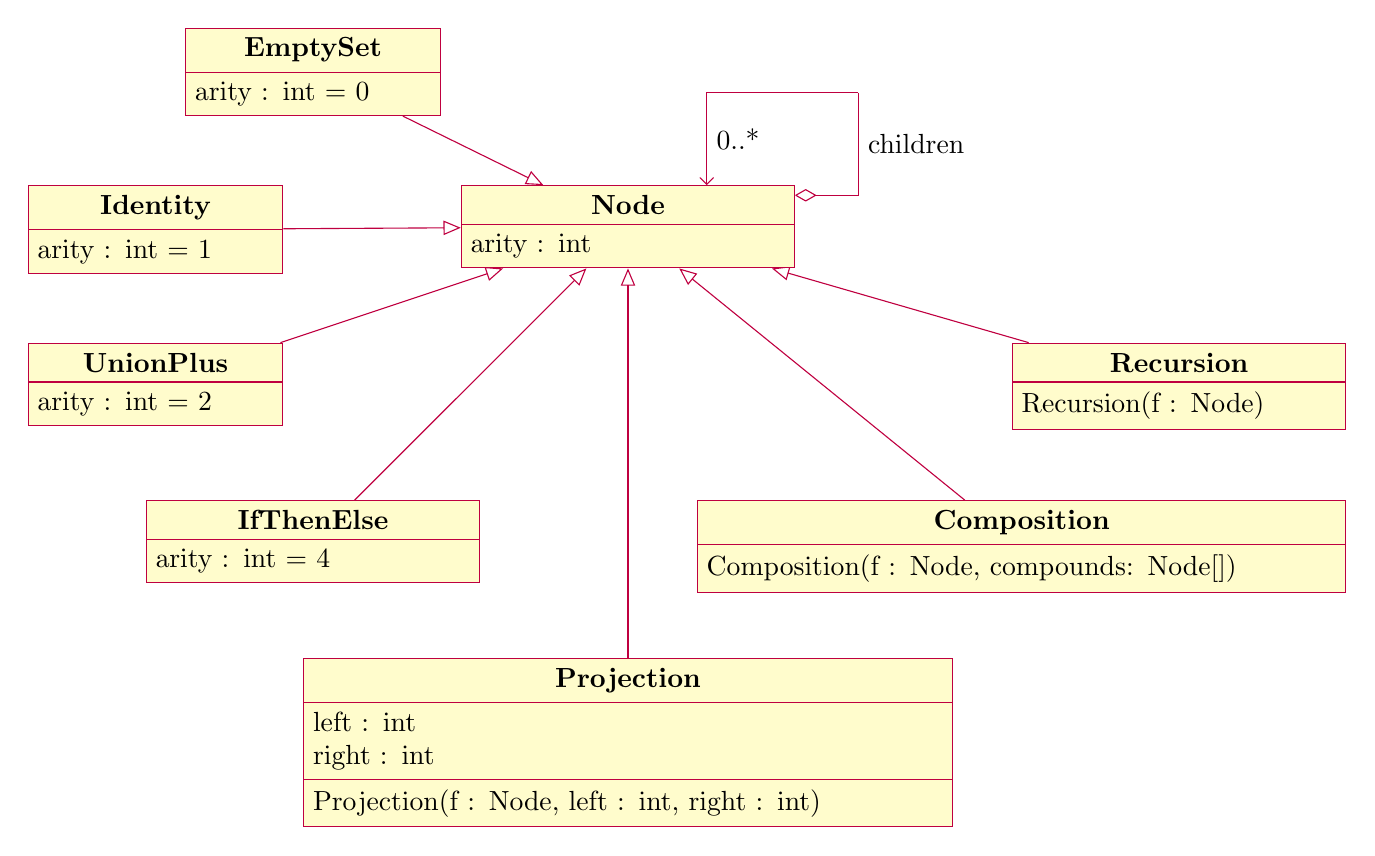
\begin{tikzpicture}
            \begin{class}[text width=4cm]{Node}{0,0}
            \attribute{arity : int}
            \end{class}
        
            \begin{class}[text width=3cm]{EmptySet}{-4,2}
            \inherit{Node}
            \attribute{arity : int = 0}
            \end{class}
        
            \begin{class}[text width=3cm]{Identity}{-6,0}
                \inherit{Node}
                \attribute{arity : int = 1}
            \end{class}

            \begin{class}[text width=3cm]{UnionPlus}{-6,-2}
                \inherit{Node}
                \attribute{arity : int = 2}
            \end{class}

            \begin{class}[text width=4cm]{IfThenElse}{-4,-4}
                \inherit{Node}
                \attribute{arity : int = 4}
            \end{class}

            \begin{class}[text width=8cm]{Composition}{5,-4}
                \inherit{Node}
                \operation{Composition(f : Node, compounds: Node[])}
            \end{class}

            \begin{class}[text width=4cm]{Recursion}{7,-2}
                \inherit{Node}
                \operation{Recursion(f : Node)}
            \end{class}

            \begin{class}[text width=8cm]{Projection}{0,-6}
                \inherit{Node}
                \attribute{left : int}
                \attribute{right : int}
                \operation{Projection(f : Node, left : int, right : int)}
            \end{class}

            \draw [umlcd style,fill=none,open diamond-] ([yshift=0.4cm]Node.east) -| ++(0.8,1.3cm)
            coordinate (tmp)
            node[right,near end] {children};
            \draw [umlcd style,fill=none,->] (tmp) -| ([xshift=1cm] Node.north)
            node[near end, right] {0..*};
        \end{tikzpicture}
    }

    \caption{Représentation UML des noeuds}
    \label{fig:uml nodes}
\end{figure}

Remarquons qu'à partir de l'arbre syntaxique généré, on peut déjà vérifier la validité du programme
en contrôlant les arités de chaque noeud de l'arbre. 

\subsubsection{Interprétation de l'arbre syntaxique}

Pour pouvoir interpréter un programme, nous allons devoir parcourir l'arbre
syntaxique qui lui est associé. Pour cela, nous allons mettre en place un patron de conception
visiteur.

\begin{figure}[H]
    \fbox{
        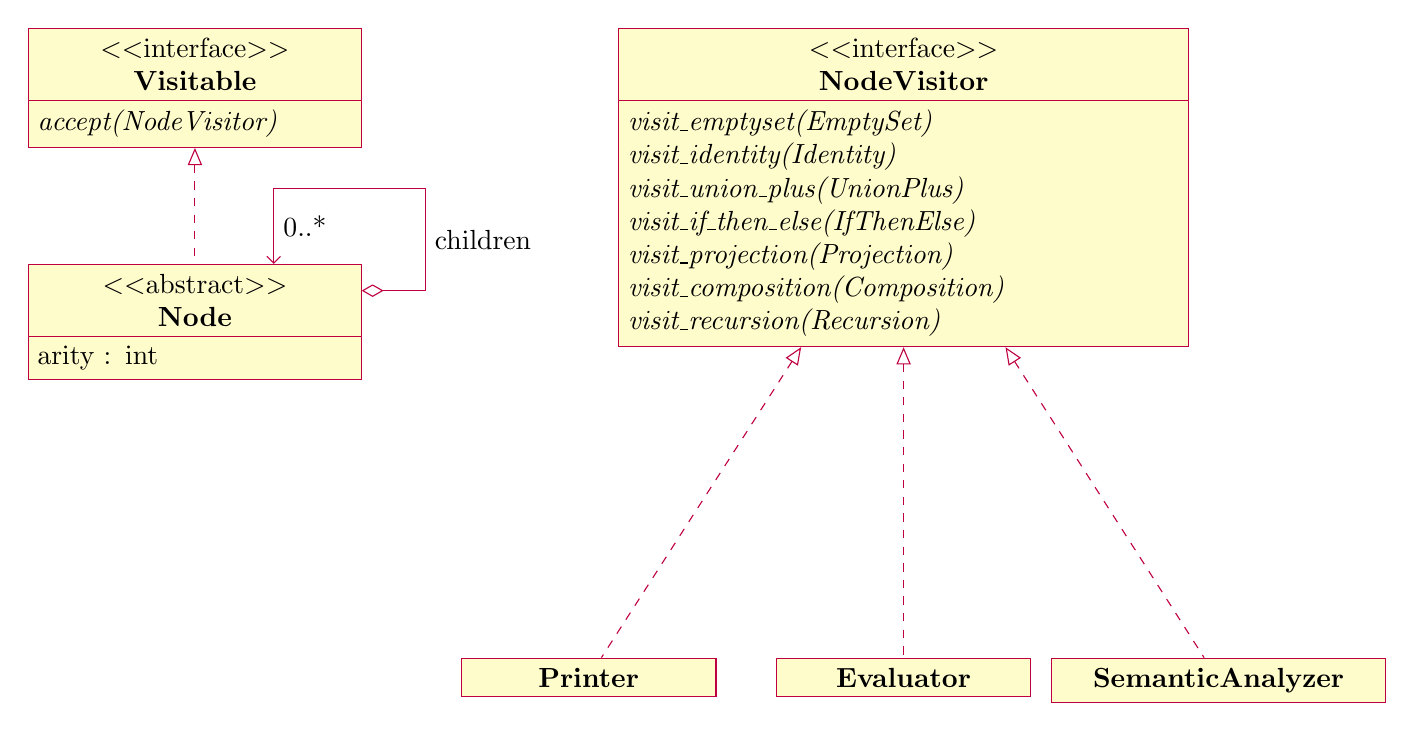
\begin{tikzpicture}
            \begin{interface}[text width=4cm]{Visitable}{0,3}
                \operation[0]{accept(NodeVisitor)}
            \end{interface}

            \begin{abstractclass}[text width=4cm]{Node}{0,0}
            \implement{Visitable}
            \attribute{arity : int}
            \end{abstractclass}

            \begin{interface}[text width=7cm]{NodeVisitor}{9,3}
                \operation[0]{visit\_emptyset(EmptySet)}
                \operation[0]{visit\_identity(Identity)}
                \operation[0]{visit\_union\_plus(UnionPlus)}
                \operation[0]{visit\_if\_then\_else(IfThenElse)}
                \operation[0]{visit\_projection(Projection)}
                \operation[0]{visit\_composition(Composition)}
                \operation[0]{visit\_recursion(Recursion)}
            \end{interface}
 
            \begin{class}[text width=3cm]{Printer}{5,-5}
                \implement{NodeVisitor}
            \end{class}

            \begin{class}[text width=3cm]{Evaluator}{9,-5}
                \implement{NodeVisitor}
            \end{class}

            \begin{class}[text width=4cm]{SemanticAnalyzer}{13,-5}
                \implement{NodeVisitor}
            \end{class}

            \draw [umlcd style,fill=none,open diamond-] ([yshift=0.4cm]Node.east) -| ++(0.8,1.3cm)
            coordinate (tmp)
            node[right,near end] {children};
            \draw [umlcd style,fill=none,->] (tmp) -| ([xshift=1cm] Node.north)
            node[near end, right] {0..*};
        \end{tikzpicture}
    }

    \caption{UML patron de conception visiteur}
    \label{fig:uml visitor pattern}
\end{figure}

Il est important de remarquer que ce patron de conception nous permet 
également de pouvoir représenter l'arbre
sous diverses formes ou bien d'effectuer son analyse sémantique 
sans avoir à modifier la base de code actuelle.

Pour pouvoir évaluer chaque noeud, nous avons ajouté la notion d'expression
qui permet d'ajouter l'appel d'un noeud avec ses arguments à la pile d'exécution.

On a choisi d'utiliser des expressions paresseuses (voir figure \ref{fig:uml expressions}) 
par souci de performances. Ainsi, on évalue une expression seulement si le résultat
est nécessaire pour continuer l'exécution du programme. Les expressions paresseuses 
sont mutables et sont closes lorsqu'elles sont évaluées. Ainsi, le résultat de 
l'évaluation d'une expression est propagé dans toutes les expressions qui la contenaient.
Lors de l'appel initial de l'interpréteur, celui-ci crée des expressions qui sont forcement 
closes puisqu'elles
contiennent les valeurs des paramètres fournis par l'utilisateur.


\begin{figure}[H]
    \fbox{
        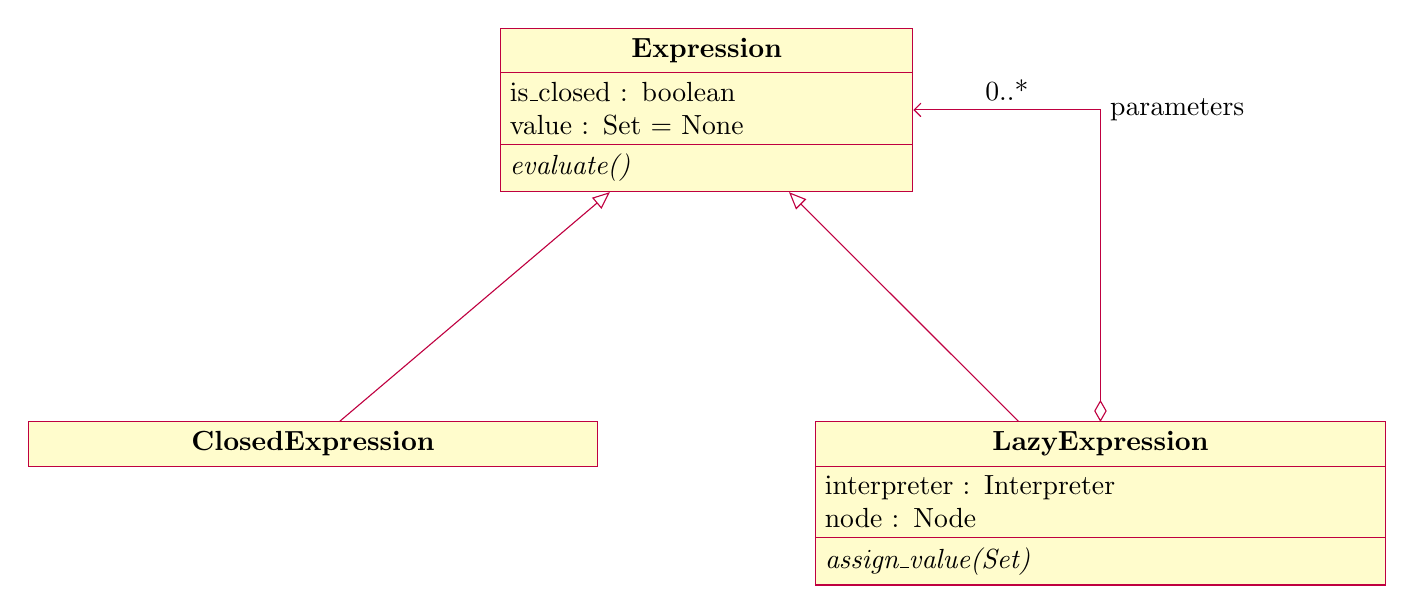
\begin{tikzpicture}
            \begin{class}[text width=5cm]{Expression}{0,0}
            \attribute{is\_closed : boolean}
            \attribute{value : Set = None}
        
            \operation[0]{evaluate()}
            \end{class}
        
            \begin{class}[text width=7cm]{ClosedExpression}{-5,-5}
            \inherit{Expression}
            \end{class}
        
            \begin{class}[text width=7cm]{LazyExpression}{5,-5}
                \inherit{Expression}
                \attribute{interpreter : Interpreter}
                \attribute{node : Node}
                \operation[0]{assign\_value(Set)}
            \end{class}
        
            \draw [umlcd style,fill=none,open diamond->] (LazyExpression.north) |- (Expression.east)
            node[right,midway] {parameters} node[near end, above] {0..*};
        \end{tikzpicture}
    }

    \caption{Représentation UML des expressions}
    \label{fig:uml expressions}
\end{figure}


Lorsqu'une expression doit être évaluée, l'interpreteur fait appel au visiteur 
\lstinline{Evaluator} pour évaluer le résultat d'un noeud sur les paramètres de
l'expression parente.

Par exemple, prenons l'expression E qui contient le noeud \lstinline{Identity}
noté I et une expression en paramètre P. Pour évaluer E, nous avons deux 
possibilités: 

\begin{itemize}
    \item soit P est close et dans ce cas, on peut clore E en lui assignant la valeur de P;
    \item soit P n'est pas close et dans ce cas, on l'ajoute à la pile d'exécution.
    P sera alors évaluée jusqu'à être close, puis l'expression E sera de nouveau
    évaluée et la valeur de P lui sera assignée.
\end{itemize}

Il en est de même pour les noeuds \lstinline{EmptySet}, \lstinline{UnionPlus},
\lstinline{IfThenElse} et \lstinline{Projection}.
Le noeud \lstinline{Composition} est un peu particulier car il ajoute 
une nouvelle expression sur la pile qui possède le noeud f et n nouvelles 
expressions en paramètres correspondants au n composantes.

Enfin, le noeud \lstinline{Recursion} nécessite d'ajouter un noeud 
qui permet d'effectuer l'opération 
$\displaystyle\bigcup_{u \in x} f(u)$ uniquement si l'évaluation de cette union
est nécessaire. Pour cela, nous avons besoin d'un noeud noté 
\lstinline{Union} qui évaluera chacun des $f(u)$ et un autre noeud noté 
\lstinline{Merge} qui construira l'union des $f(u)$.

\begin{figure}[H]
    \fbox{
        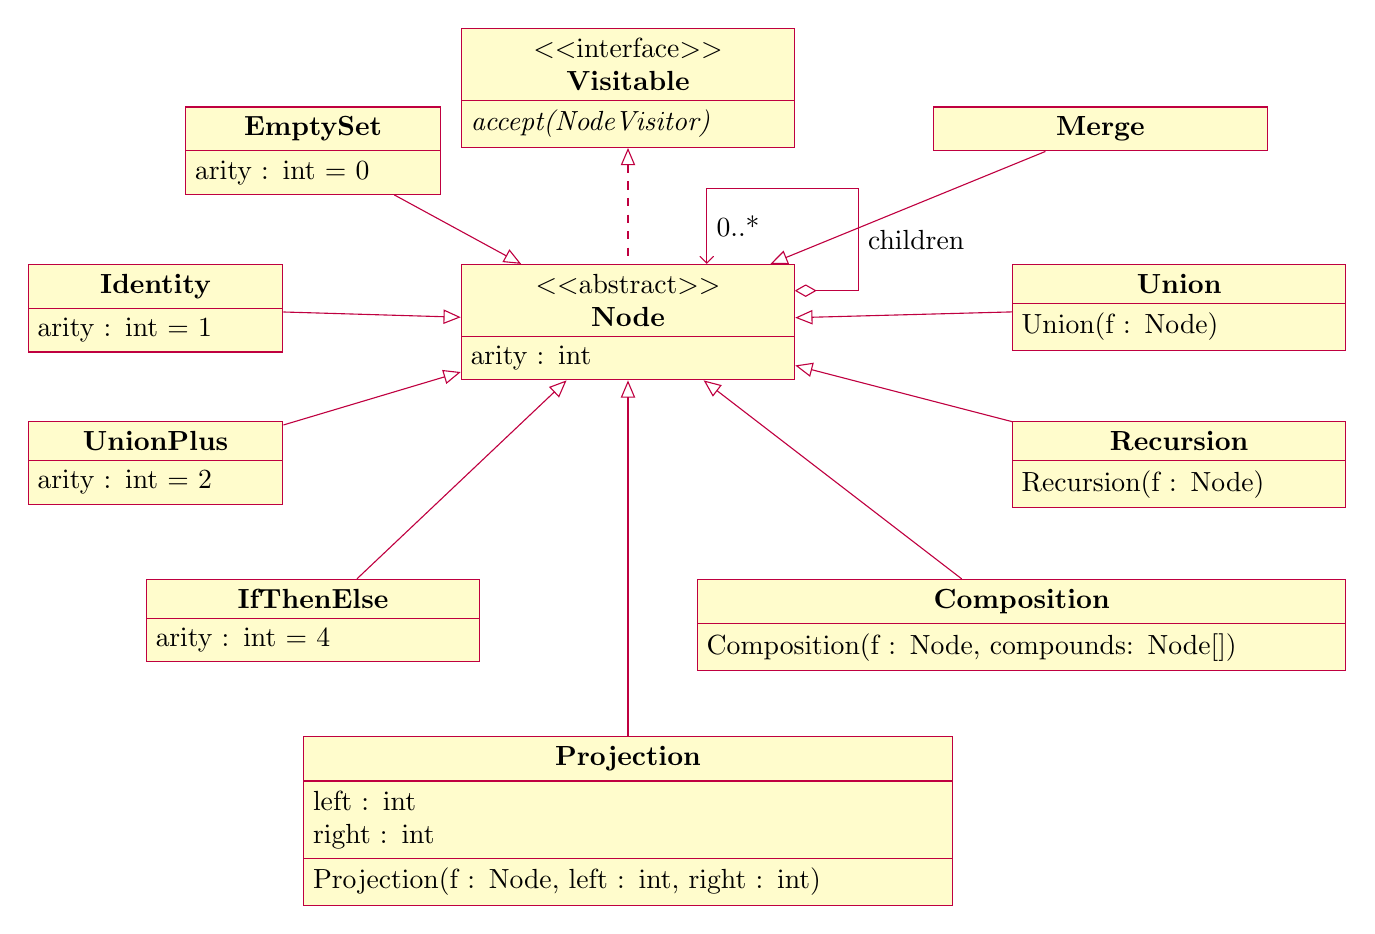
\begin{tikzpicture}
            \begin{interface}[text width=4cm]{Visitable}{0,3}
                \operation[0]{accept(NodeVisitor)}
            \end{interface}

            \begin{abstractclass}[text width=4cm]{Node}{0,0}
            \implement{Visitable}
            \attribute{arity : int}
            \end{abstractclass}
        
            \begin{class}[text width=3cm]{EmptySet}{-4,2}
            \inherit{Node}
            \attribute{arity : int = 0}
            \end{class}
        
            \begin{class}[text width=3cm]{Identity}{-6,0}
                \inherit{Node}
                \attribute{arity : int = 1}
            \end{class}

            \begin{class}[text width=3cm]{UnionPlus}{-6,-2}
                \inherit{Node}
                \attribute{arity : int = 2}
            \end{class}

            \begin{class}[text width=4cm]{IfThenElse}{-4,-4}
                \inherit{Node}
                \attribute{arity : int = 4}
            \end{class}

            \begin{class}[text width=8cm]{Composition}{5,-4}
                \inherit{Node}
                \operation{Composition(f : Node, compounds: Node[])}
            \end{class}

            \begin{class}[text width=4cm]{Recursion}{7,-2}
                \inherit{Node}
                \operation{Recursion(f : Node)}
            \end{class}

            \begin{class}[text width=4cm]{Union}{7,0}
                \inherit{Node}
                \operation{Union(f : Node)}
            \end{class}

            \begin{class}[text width=4cm]{Merge}{6,2}
                \inherit{Node}
            \end{class}

            \begin{class}[text width=8cm]{Projection}{0,-6}
                \inherit{Node}
                \attribute{left : int}
                \attribute{right : int}
                \operation{Projection(f : Node, left : int, right : int)}
            \end{class}

            \draw [umlcd style,fill=none,open diamond-] ([yshift=0.4cm]Node.east) -| ++(0.8,1.3cm)
            coordinate (tmp)
            node[right,near end] {children};
            \draw [umlcd style,fill=none,->] (tmp) -| ([xshift=1cm] Node.north)
            node[near end, right] {0..*};
        \end{tikzpicture}
    }

    \caption{Représentation UML des noeuds avec Union et Merge}
    \label{fig:uml nodes complete}
\end{figure}


Plus tôt, dans la partie \ref{arbre syntaxique}, nous avons
expliqué la mise en cache des noeuds mais cette explication était incomplète.
En effet, la mise en cache des noeuds devient très intéressante pour l'évaluateur,
puisque lorsqu'une expression sera évaluée, on met en cache son résultat pour accélérer
le calcul des autres expressions (par exemple dans le cas d'un calcul de la fonction
de Fibonacci). Cette mise en cache nécessite de comparer les expressions deux à deux
et cette comparaison nécessite de comparer les noeuds. Sans mise en cache, comparer deux
noeuds peut être long car nous devons comparer tous les descendants de chaque noeud, or
avec la mise en cache, il suffit de comparer les adresses mémoires pour comparer les noeuds.

Pour finir, l'interpréteur utilise des ensembles immutable
comme élément du modèle. L'immutabilité permet de
factoriser la taille en mémoire des grands ensembles, en particulier pour les ordinaux.
Par exemple, l'ordinal $n$ contient $n$ ordinaux de $0$ à $n-1$. Au total, l'ordinal
$n$, représenté sous forme d'arbre, contient $2^n$ sommets, mais seulement $n+1$ éléments
distincts. On peut donc gagner beaucoup de mémoire en réutilisant les ensembles
précédemment construits.

\subsubsection{Fonctions}

Pour compléter l'interpréteur, nous avons ajouté un type de noeuds
qui contient son propre comportement (au lieu que celui-ci soit inclus dans
l'évaluateur). 
Cela nous permet de définir des fonctions qui remplacent certains programmes.

\paragraph{Exemple} Le programme \progS{R>I} est le programme $(x) \mapsto 0$.
Ce programme n'est pas très intéressant, d'autant plus que le programme \progS{>E} 
est équivalent et plus court. Sauf que le programme \progS{R>I} nécessite n étapes
de calculs où n est le rang de $x$. On se trouve donc face à un programme couteux à exécuter
pour finalement aboutir à un résultat simple à calculer.
D'autres exemples existent comme \progS{RR?} qui est encore plus long à évaluer
et qui calcul $(x, y) \mapsto 0$.

Pour ce type de programme, les fonctions permettent de précompiler leurs comportements.

\subsection{Générateur}

Le générateur de programmes a pour but de nous aider à identifier et 
déterminer le comportement des programmes de petite taille. Le travail 
d'analyse des programmes devra être manuel, mais il permettra de fortement
améliorer les performances de l'interpréteur en précompilant le comportement
des petits programmes.

Le générateur est une fonction $G$ à 2 arguments: la taille $n$ du programme 
voulu et son arité $a$. Par conséquent, $G(n, a)$ renvoie l'ensemble des 
programmes de taille $n$ et d'arité $a$.

\def\fprime{\mbox{\scriptsize\bfseries $f'$}}
\def\gnmoinsun{\mbox{\scriptsize\bfseries $g_{n\text{-}1}$}}

Pour l'implémentation, nous avons construit une fonction $G$ qui prend en argument
3 paramètres: la taille $n$, l'arité $a$ et un troisième paramètre permettant de
ne pas inclure de jetons \progS{<} ou \progS{>} au résultat. Ce choix vient du 
fait que l'on veut minimiser la génération de programme existant sous une forme
plus courte. Dans le cas de la composition, si on a \progS{o<!f!\gone!\dots!\gn}
alors on peut construire un programme plus court équivalent:
\progS{o!f!\gtwo!\dots!\gn}. De même avec \progS{o>!f!\gone!\dots!\gn}, on aurait
\progS{o!f!\gone!\dots!\gnmoinsun} qui serait plus court et équivalent.
On élimine également le cas inverse dans lequel toutes les composantes commencent
par \progS{<} ou \progS{>} car \progS{o!f>!\gone!\dots>!\gn} = \progS{>o!f!\gone!\dots!\gn}
qui est plus court dès que $n > 1$.
Pour la récursion, on a \progS{R<!p} qui est équivalent à \progS{!p} et,
dans le cas ou \progS{!p} est d'arité $n > 1$, on a \progS{>R!p} qui équivaut à
\progS{R>!p}.


\subsection{Benchmark}

Lors de l'énumération des programmes, nous avons découvert des programmes de même taille calculant
la même fonction. Un des points que nous souhaitions analyser est le nombre d'étape de calcul
de chaque programme sur certaines entrées. Pour ce faire, nous avons développé un outil de benchmark
qui compte le nombre d'étape de calcul atomiques: les fonctions initiales correspondant aux jetons
\progS{E+?}. Les résultats sont
sauvegardés sous forme de tableau puis le coefficient directeur de la courbe associé est calculé.

Le développement du benchmark a nécessité de revoir l'implémentation de la mise en cache des expressions.
La mise en cache des expressions fait partie intégrante de l'interpréteur et le nombre d'étapes
sans mise en cache devient tellement élevé que les mesures sur certains programmes deviennent impossibles.
Nous devions donc utiliser la mise en cache des expressions durant les mesures mais tout en réinitialisant
le cache entre chaque calcul pour éviter de fausser les données. Nous avions alors deux choix possibles:
\begin{itemize}
    \item forcer une réinitialisation du cache entre chaque calcul lors des mesures sans modifier le
    comportement actuel de la mise en cache des expressions.
    \item contextualiser la mise en cache des expressions à chaque nouveau calcul. C'est-à-dire que 
    chaque calcul dispose de son propre cache.
\end{itemize}

La première solution utilise plus de mémoire vive car tous les calculs sont conservés mais lorsque l'on effectue
deux fois le même calcul, la seconde fois ne nécessite qu'un appel au cache.
La seconde solution utilise un cache pour les expressions uniquement durant le calcul de celle-ci.
L'usage de la mémoire vive est donc grandement diminué et on a l'avantage/inconvénient qu'effectuer
deux fois le même calcul nécessitera le même nombres d'étape de calcul. Ce deuxième point est nuancé car
on effectue rarement deux fois le même calcul dans la pratique. De plus, ne pas avoir de cache partagé
est justement nécessaire pour effectuer des mesures pertinentes pour notre benchmark.

Pour finir, dans le premier
cas, il faut garder une trace des calculs qui auraient pu être interrompus par l'utilisateur. Ces calculs,
à cause de l'intervention de l'utilisateur, restent sans résultats mais sont pourtant conservés en mémoire.
Ils font donc garder une trace des ajouts dans le cache lors d'un calcul pour les supprimer en cas de problème.
Ce problème couplé à l'importante charge que subit la mémoire vive pose de gros problèmes de performance en
cas d'interruption de l'interpréteur.

Pour toutes ces raisons, nous avons décidé de modifier le comportement actuel de la mise en cache des expressions
en optant pour la deuxième solution: contextualiser la mise en cache des expressions à chaque nouveau calcul.

Remarquons que les autres caches (celui des ensembles et celui des noeuds) ne nécessitent aucune modification.
Le benchmark compte le nombre d'appels aux jetons atomiques, ces deux autres caches n'ont donc aucun
impact sur le résultat.

\subsubsection{Exemples}

\paragraph{clôture transitive}

On s'intéresse ici à l'étude du programme \progS{R+}. Le nombre d'étapes étant linéaire dans ce cas,
nous affichons également un graphique sans échelle logarithmique.

\begin{figure}[h]
    \fbox{
    \begin{subfigure}{0.5\textwidth}
        
            \includegraphics[width=\linewidth, left]{benchmark_R+_logscale.png}
        
        \caption{Benchmark de \progS{R+} en échelle logarithmique}
        \label{benchmark transitive closure log scale}
    \end{subfigure}
    \begin{subfigure}{0.5\textwidth}

            \includegraphics[width=\linewidth, right]{benchmark_R+_regularscale.png}
        
        \caption{Benchmark de \progS{R+} en échelle classique}
        \label{benchmark transitive closure regular scale}
    \end{subfigure}
    }
\end{figure}

\`{A} partir de la figure \ref{benchmark transitive closure log scale}, on déduit que le programme
\progS{R+} est linéaire par rapport au rang de l'entrée. Pour l'exemple, on décide de tracer la courbe
en échelle classique pour visualiser le coefficient de la fonction affine obtenue en figure
\ref{benchmark transitive closure regular scale}.

On peut illustrer l'impact du cache en affichant la courbe obtenue lorsque la mise en cache 
des expressions est désactivée.

\begin{figure}[H]
        \begin{center}
            \fbox{
                \includegraphics[width=0.7\linewidth]{benchmark_R+_logscale_nocache.png}
            }
        \end{center}
        \caption{Benchmark de \protect\progS{R+} en échelle logarithmique sans mise en cache}
        \label{benchmark transitive closure log scale no cache}
\end{figure}

Sans la mise en cache, il devient difficile d'effectuer des mesures, même pour un programme 
aussi simple que la clôture transitive. 
Le nombre d'étapes nécessaire est exponentiel, et remarquons qu'avec le cache, nous pouvions
faire des mesures sur des ensembles de rang 50 en moins de 100 étapes tandis que sans la mise en cache,
la clôture transitive nécessite plus d'un million d'étapes de calcul dès le rang 20.

\paragraph{Multiplication}

On s'intéresse ici à l'étude du programme \progS{'\mult}.

\begin{figure}[H]
        \begin{center}
            \fbox{
                \includegraphics[width=0.7\linewidth]{benchmark_mult_logarithmicscale.png}
            }
            \caption{Benchmark de \protect\progS{'\mult} en échelle logarithmique}
        \end{center}
\end{figure}

La multiplication est un programme d'arité 2, en conséquence, on s'intéresse à l'évolution
du nombre d'étapes de calcul en fonction de chacun des paramètres. Dans cet exemple, le coefficient
du nombre d'étapes en fonction de $x$ (le premier paramètre) est de $1.108$ tandis qu'il est de $1.493$
par rapport à $y$ (le deuxième paramètre).

\subsubsection{Outil de comparaison} 

Pour faciliter la visualisation des données, on propose de réunir les
résultats de plusieurs programmes sur la même figure.

On s'intéresse ici à la fonction successeur sur les ordinaux \progS{'\successeur} = \progS{o+II}.
On verra dans la section \ref{lemme:preuve rplus egal successeur} que la clôture transitive \progS{R+}
se comporte comme la fonction successeur \progS{'\successeur}. 
On cherche donc à comparer la complexité de ces deux programmes pour déterminer le plus performant.

\begin{figure}[H]
        \begin{center}
            \fbox{
                \includegraphics[width=0.7\linewidth]{constant_vs_lin.png}
            }
            \caption{Comparatif de \protect\progS{o+II} et \protect\progS{R+} en échelle logarithmique}
        \end{center}
\end{figure}

Comme le programme \progS{o+II} ne comporte aucun jeton \progS{R}, le nombre d'étapes de calcul 
de ce programme est constant par rapport à l'entrée. Cela correspond au coefficient $0$ de la courbe
en échelle logarithmique.

En revanche, le programme \progS{R+} quant à lui opère une récursion sur l'entrée. Ce programme effectue donc un nombre d'étapes qui
dépend de la taille de l'entrée. En l'occurrence, comme le coefficient en échelle logarithmique est de $1$, le nombre d'étapes est linéairement
proportionnel à la taille de l'entrée.

Cet outil nous permet ainsi de visualiser rapidement les fonctions donc la complexité est trop grande
pour être analysé via les outils développés.

Un exemple de ce genre de programme est \progS{R>R>Ro+++}:

\begin{figure}[H]
        \begin{center}
            \fbox{
                \includegraphics[width=0.7\linewidth]{compare_exp_lin.png}
            }
            \caption{Benchmark de \protect\progS{R>R>Ro+++} avec \protect\progS{R>Ro+++} comme référence en échelle logarithmique}
        \end{center}
\end{figure}

Sur cette figure, le programme \progS{R>Ro+++} est en complexité linéaire par rapport à l'entrée.
En comparaison, la courbe du programme \progS{R>R>Ro+++} correspond à celle d'une exponentielle
 en échelle logarithmique. Et en effet, le programme \progS{R>R>Ro+++} calcul la fonction
$(x) \mapsto 2^x - 2$, impliquant que ce programme est, à minima, en complexité exponentielle par rapport
à l'entrée.

\subsection{Programmes générés \label{programmes generes}}

Dans cette section, nous présentons les résultats obtenue lors de l'énumération des petits programmes.
Cette énumération permet  d’accélérer l’étude des programmes plus grands et de comprendre à partir 
de quelle taille de programmes certains comportements complexes apparaissent naturellement dans notre modèle de
calcul.

\subsubsection{Taille 2}

\begin{enumerate}
    \item \progS{R+} = \progS{'\tc}: $(x) \mapsto TC(\{x\})$
    \begin{lemma} \label{lemme:ensemble transitif contient cloture transitive de ses elements}
        Un ensemble transitif contient les clôtures transitives de ses éléments.
    \end{lemma}
    \begin{proof} Soit $\alpha$ un ensemble transitif, on a
        \[
            \forall u \in \alpha, cloture(u) \subset \alpha
        \] donc 
        \[
            \bigcup_{u \in \alpha} cloture(u) \subset \alpha
        \]
    \end{proof}
    \begin{lemma} \label{lemme:preuve rplus egal successeur}
        $\progS{R+}(\alpha) = \progS{'\successeur}(\alpha)$ dans le cas où $\alpha$ est transitif
    \end{lemma}
    \begin{proof}
        Soit $\alpha$ un ensemble transitif, alors $\displaystyle\bigcup_{u \in \alpha} \progS{R+}(u) \subset \alpha$, d'après le lemme \ref{lemme:ensemble transitif contient cloture transitive de ses elements}.
            Réciproquement, $\forall u \in \alpha, u \in \progS{R+}(u)$ donc on a $\alpha \subset \displaystyle\bigcup_{u \in \alpha} \progS{R+}(u)$.
            On en déduit que $\displaystyle\bigcup_{u \in \alpha} \progS{R+}(u) = \alpha$.
            Ce qui nous donne:
            \begin{align*} 
                \progS{R+}(\alpha) &= \displaystyle\bigcup_{u \in \alpha} \progS{R+}(u) \cup \{\alpha\} \\
                &= \progS{'\successeur}(\alpha) \\
            \end{align*}
    \end{proof}
    \item \progS{R?}: $(x, y, z) \mapsto \emptyset \mbox{ si } y \in z \mbox{ sinon } x$
\end{enumerate}

\subsubsection{Taille 4}

\begin{enumerate}
    \item \progS{o+EE}: $() \mapsto 1$
    \item \progS{R>R+}: $(x) \mapsto rang(x) + 1$
    \item \progS{o+II} = \progS{'\successeur}: $(x) \mapsto x \cup \{x\} = S(x)$

    \item \progS{o+++}: $(x, y) \mapsto x \cup \{y, x \cup \{y\}\}$
    \begin{figure}[H]
        \fboxsep=5mm
        \centering\fbox{
            \begin{tikzpicture}[
                sibling distance=5cm, 
                level 2/.style={sibling distance =2cm},
                subset1/.style={draw,dashed,shape border uses incircle,
                isosceles triangle,isosceles triangle apex angle=150,
                shape border rotate=-75,yshift=0.25cm, xshift=2cm,
                minimum height=0.8cm},
                subset2/.style={draw,dashed,shape border uses incircle,
                isosceles triangle,isosceles triangle apex angle=110,
                shape border rotate=-55,yshift=0.3cm, xshift=0cm,
                minimum height=0.9cm},
                ]
                \node [] {$\bigdot$}
                    child{ node[subset1] {$x$} edge from parent[draw=none] }
                    child {node[] {$y$} }
                    child { node [] {$\bigdot$}
                            child{ node[subset2] {$x$}  edge from parent[draw=none] }
                            child {node[] {$y$} }
                        };
            \end{tikzpicture}
        }
    \end{figure}
    \item \progS{oR++}: $(x, y) \mapsto TC(\{x \cup \{y\}\})$
    \item \progS{o+??}: $(x, y, u, v) \mapsto S(x) \mbox{ si } u \in v \mbox{ sinon } S(y)$
    \item \progS{oR+?}: $(x, y, u, v) \mapsto TC(x) \mbox{ si } u \in v \mbox{ sinon } TC(y)$
\end{enumerate}

\subsubsection{Taille 5}

\def\roplusplusplus{\mbox{\scriptsize\bfseries $++$}}

\begin{enumerate}
    \item \progS{Ro+++} = \progS{RoR++} = \progS{'\roplusplusplus}: $(x) \mapsto TC(\{\displaystyle\bigcup_{u \in x} (\progS{'\roplusplusplus}(u)) \cup \{x\}\})$
    \begin{proof}[\textbf{Preuve de \progS{Ro+++} = \progS{RoR++} par récurrence transfinie:}]
        $ $\newline
        Pour cette preuve, nous allons également vérifier que pour tout ensemble $\alpha$, \[
         \progS{Ro+++}(\alpha) = \progS{RoR++}(\alpha)  \mbox{ est un ensemble transitif.} \]
        \begin{itemize}
            \item \progS{Ro+++}(0) = \progS{RoR++}(0) = 2, et comme 2 est un ordinal, il est transitif.
            \item Soit $\alpha$ un ensemble, on suppose que pour tout $u \in \alpha$, on a: \[
                \progS{Ro+++}(u) = \progS{RoR++}(u) = P(u) \mbox{ et P(u) est un ensemble transitif}\]
            Alors
            \begin{align*} 
                \progS{Ro+++}(\alpha) &= \progS{o+++}(\displaystyle\bigcup_{u \in \alpha} \progS{Ro+++}(u), \alpha) \\ 
                &= \progS{o+++}(\displaystyle\bigcup_{u \in \alpha} P(u), \alpha) \tag*{Par hypothèse de récurrence} \\
                &= \displaystyle\bigcup_{u \in \alpha} P(u) \cup \{\alpha, \displaystyle\bigcup_{u \in \alpha} P(u) \cup \{\alpha\}\} \\
                &= \progS{'\successeur}(\displaystyle\bigcup_{u \in \alpha} P(u) \cup \{\alpha\}) \\
            \end{align*}
            \begin{align*} 
                \progS{RoR++}(\alpha) &= \progS{oR++}(\displaystyle\bigcup_{u \in \alpha} \progS{RoR++}(u), \alpha) \\ 
                &= \progS{oR++}(\displaystyle\bigcup_{u \in \alpha} P(u), \alpha) \tag*{Par hypothèse de récurrence} \\
                &= TC(\{\displaystyle\bigcup_{u \in \alpha} P(u) \cup \{\alpha\}\}) \\
            \end{align*}
            Comme $\forall u \in \alpha, P(u)$ est transitif, alors $\displaystyle\bigcup_{u \in \alpha} P(u)$ est transitif.
            De plus, comme $\forall u \in \alpha$, on a $u \in P(u)$ alors $\displaystyle\bigcup_{u \in \alpha} P(u) \cup \{\alpha\}$ est transitif.
            Or sur un ensemble transitif, d'après le lemme \ref{lemme:preuve rplus egal successeur}, on sait que \progS{R+} = \progS{'\successeur}.
            Finalement, on a donc :
            \begin{align*} 
                \progS{RoR++}(\alpha) &= \progS{'\successeur}(\{\displaystyle\bigcup_{u \in \alpha} P(u) \cup \{\alpha\}\}) \\
                &= \progS{Ro+++}(\alpha)
            \end{align*}
        \end{itemize}
    \end{proof}

    \paragraph{Exemple:} $\progS{Ro+++}(\{\{1\}\})$

    \begin{figure}[H]
        \fboxsep=5mm
        \centering\fbox{
            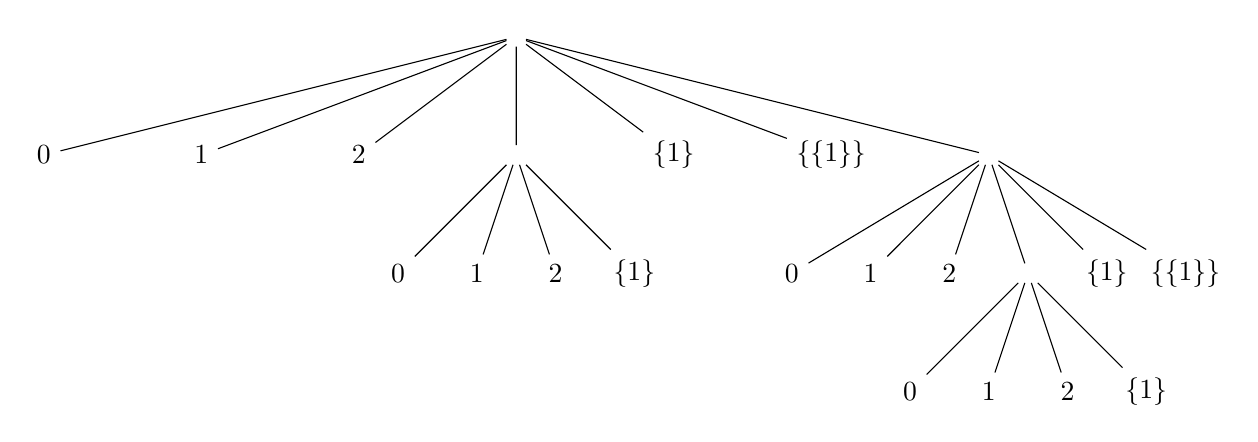
\begin{tikzpicture}[
                sibling distance=2cm, 
                level 2/.style={sibling distance =1cm},
                triangle/.style={isosceles triangle,draw,shape border rotate=90, dashed, minimum height=10mm, minimum width=15mm, inner sep=0},
                ]
                \node [] {$\bigdot$}
                    child{ node[] {0} }
                    child{ node[] {1} }
                    child{ node[] {2} }
                    child { node [] {$\bigdot$}
                        child{ node[] {0} }
                        child{ node[] {1} }
                        child{ node[] {2} }
                        child{ node[] {\{1\}} }
                    }
                    child{ node[] {\{1\}} }
                    child{ node[] {\{\{1\}\}} }
                    child { node [] {$\bigdot$}
                        child{ node[] {0} }
                        child{ node[] {1} }
                        child{ node[] {2} }
                        child { node [] {$\bigdot$}
                            child{ node[] {0} }
                            child{ node[] {1} }
                            child{ node[] {2} }
                            child{ node[] {\{1\}} }
                        }
                        child{ node[] {\{1\}} }
                        child{ node[] {\{\{1\}\}} }
                    };
            \end{tikzpicture}
        }
    \end{figure}

\paragraph{Étude de complexité} \mbox{} \\

\begin{minipage}{\linewidth}
    \begin{figure}[H]
            \begin{center}
                \fbox{
                    \includegraphics[width=0.7\linewidth]{comparison_Ro+++_RoR++.png}
                }
            \end{center}
        \caption{Comparaison de \protect\progS{Ro+++} et de \protect\progS{RoR++} en échelle logarithmique}
    \end{figure}
\end{minipage}


    On peut observer sur ce graphique que les deux droites sont parallèles (même coefficient directeur),
    ce qui indique que les deux programmes sont de même complexité. Le coefficient étant de $1$,
     cette complexité est linéaire. Cependant, l'écart entre les courbes indique qu'il existe un facteur
     entre le nombre d'étapes nécessaires pour chaque programme. En l'occurrence, le programme \progS{RoR++}
     nécessite $1.5$ fois plus d'étapes que le programme \progS{Ro+++}.

    De ce fait, comme ces deux programmes calculent la même fonction, par la suite, nous utiliserons 
    le programme \progS{Ro+++}. 
    (Ce qui signifie que le programme \progS{R>Ro+++} sera généré mais pas le programme \progS{R>RoR++})

    \item \progS{o+I<E}: $(x) \mapsto x \cup \{0\}$
    \item \progS{o+IR+}: $(x) \mapsto x \cup \{TC(\{x\})\}$
    \item \progS{o+<EI} = \progS{'\singleton}: $(x) \mapsto \{x\}$
    \item \progS{oR+R+}: $(x) \mapsto TC(\{TC(\{x\})\}) = S(TC(\{x\}))$
    \item \progS{o++>I}: $(x, y) \mapsto x \cup \{x , y\} = S(x) \cup \{y\}$
    \item \progS{o+<I+}: $(x, y) \mapsto y \cup \{x \cup \{y\}\}$
    \item \progS{o+>I+}: $(x, y) \mapsto x \cup \{x \cup \{y\}\}$
    \item \progS{Ro+??}: $(x, u, v) \mapsto rang(x) + 1 \mbox{ si } u \in v \mbox{ sinon } S(x)$
    \item \progS{RoR+?}: $(x, u, v) \mapsto rang(x) + 1 \mbox{ si } u \in v \mbox{ sinon } TC(x)$
    \item \progS{oR+R?}: $(x, u, v) \mapsto 1 \mbox{ si } u \in v \mbox{ sinon } TC(x)$
\end{enumerate}

\subsubsection{Taille 6}

\begin{enumerate}
    \item \progS{R>R>R+} = \progS{R>o+II}: $(x) \mapsto rang(x) + 1$
    \begin{proof}[\textbf{Preuve de \progS{R>R>R+} = \progS{R>o+II} = rang + 1 par récurrence transfinie:}]
        $ $\newline
        \begin{itemize}
            \item \progS{R>R>R+}(0) = \progS{R>o+II}(0) = rang(0) + 1 = 1
            \item Soit $\alpha$ un ensemble, on suppose que pour tout $u \in \alpha$, on a: \[
                \progS{R>R>R+}(u) = \progS{R>o+II}(u) = rang(u) + 1\]
            Alors
            \begin{align*} 
                \progS{R>R>R+}(\alpha) &= \progS{R>R+}(\displaystyle\bigcup_{u \in \alpha} \progS{R>R>R+}(u)) \\ 
                &= \progS{R>R+}(\displaystyle\bigcup_{u \in \alpha} \progS{R>R>R+}(u))  \\
                &= \progS{R>R+}(\displaystyle\bigcup_{u \in \alpha} rang(u) + 1) \tag*{Par hypothèse de récurrence} \\
                &= \progS{R>R+}(rang(\alpha)) \\
                &= rang(rang(\alpha)) + 1 \tag{car \progS{R>R+} = rang + 1} \\
                &= rang(\alpha) + 1 \\
            \end{align*}
            \begin{align*} 
                \progS{R>o+II}(\alpha) &= \progS{o+II}(\displaystyle\bigcup_{u \in \alpha} \progS{R>o+II}(u)) \\ 
                &= \progS{'\successeur}(\displaystyle\bigcup_{u \in \alpha} \progS{R>o+II}(u)) \tag{car \progS{o+II} = \progS{'\successeur}} \\
                &= \progS{'\successeur}(\displaystyle\bigcup_{u \in \alpha} rang(u) + 1) \tag*{Par hypothèse de récurrence} \\
                &= \progS{'\successeur}(rang(\alpha)) \\
                &= rang(\alpha) + 1 \\
            \end{align*}
        \end{itemize}
    \end{proof}
    \newpage
    \paragraph{\'{E}tude de complexité} \mbox{} \\

    \begin{minipage}{\linewidth}
    \begin{figure}[H]
                
            \begin{center}
                \fbox{
                    \includegraphics[width=0.7\linewidth]{comparison_RrRrR+_Rro+II.png}
                }
                
            \end{center}
            \caption{Comparaison de \protect\progS{R>R>R+} et de \protect\progS{R>o+II} en échelle logarithmique}
    \end{figure}
    
\end{minipage}

Les programmes ont tous deux une complexité linéaire par rapport à l'entrée mais le programme
\progS{R>o+II} nécessite 2 fois moins d'étapes que le programme \progS{R>R>R+}.

On choisit donc de conserver le programme \progS{R>o+II} et d'ignorer le programme \progS{R>R>R+} pour
la génération de plus grands programmes.

    % \item \progS{Ro++>I}: $(x) \mapsto $
    % \item 
    % \begin{figure}[!h]
    %     \fboxsep=5mm
    %     \centering\fbox{
    %         \begin{tikzpicture}[
    %             sibling distance=3cm, 
    %             level 2/.style={sibling distance =1.8cm},
    %             triangle/.style={isosceles triangle,draw,shape border rotate=90, dashed, minimum height=10mm, minimum width=15mm, inner sep=0},
    %             ]
    %             \coordinate
    %                 child{ node[] {$S(\bigcup_{0 \leq i \leq k_0 }(a_i)) \cup \{u_0\}$}
    %                     child{ node[] {$a_0$} }
    %                     child{ node[] {$\dots$} 
    %                         child { node[] {$\vdots$} }
    %                     }
    %                     child{ node[] {$a_{k_0}$} } 
    %                 }
    %                 child{ node[] {$\dots$} }
    %                 child{ node[] {$S(\bigcup_{0 \leq i \leq k_j }(j_i)) \cup \{u_j\}$} 
    %                     child{ node[] {$j_0$} }
    %                     child{ node[] {$\dots$} 
    %                         child { node[] {$\vdots$} 
    %                             child{ node[] {$S(1) \cup \{w\}$} 
    %                                 child{ node[] {$1$} }
    %                             }
    %                         }
    %                     }
    %                     child{ node[] {$j_{n_j}$} }
    %                 }
    %                 child{ node[] {$\dots$} }
    %                 child{ node[] {$S(\bigcup_{0 \leq i \leq k_n }(z_i)) \cup \{u_n\}$}
    %                     child{ node[] {$z_0$} }
    %                     child{ node[] {$\dots$} 
    %                         child { node[] {$\vdots$} }
    %                     }
    %                     child{ node[] {$z_{k_n}$} }
    %                 };
    %         \end{tikzpicture}
    %     }
    % \end{figure}
    % \item \progS{Ro+<I+}: $(x) \mapsto$
    % \item \progS{Ro+>I+}: $(x) \mapsto$
    \item \progS{o+<ER+}: $(x) \mapsto \{TC(\{x\})\}$
    %\item \progS{RoR+R?}: $(x) \mapsto$
    \item \progS{o+<+>+}: $(x) \mapsto (x, y, z) \mapsto y \cup \{z\} \cup \{x \cup \{y\}\}$
    \item \progS{RoR+R?}: $(x, y) \mapsto rang(x') + 1, \mbox{ où } x' $ est l'ensemble $x$ dans lequel tous les éléments appartenant à $y$ sont remplacés par $0$
\end{enumerate}

\subsubsection{Taille 7}

\begin{enumerate}
    \item \begin{tabular}{lcl} \label{2 fois rang plus 2}
        \progS{R>Ro+++} & $:$ & $(x) \mapsto 2 \times rang(x) + 2$ \\
        & $=$ & \progS{R>oR+R+} \\
    \end{tabular}
    \begin{proof}[\textbf{Preuve de \ref{2 fois rang plus 2} par récurrence transfinie:}]
        $ $\newline
        \begin{itemize}
            \item \begin{align*} 
                2 \times rang(0) + 2 &= 2 \\ 
                &= \progS{R>Ro+++}(0) \\
                &= \progS{R>oR+R+}(0) \\
            \end{align*}
            \item Soit $\alpha$ un ensemble, on suppose que pour tout $u \in \alpha$, on a: 
            \begin{align*} 
                2 \times rang(u) + 2 &= \progS{R>Ro+++}(u) \\ 
                &= \progS{R>oR+R+}(u) \\
            \end{align*}
            Alors
            \begin{align*} 
                \progS{R>Ro+++}(\alpha) &= \progS{Ro+++}(\displaystyle\bigcup_{u \in \alpha} \progS{R>Ro+++}(u)) \\ 
                &= \progS{Ro+++}(\displaystyle\bigcup_{u \in \alpha} 2 \times rang(u) + 2) \tag*{Par H.R} \\
                &= \progS{Ro+++}(2 \times rang(\alpha)) \\
                &= 2 \times rang(\alpha) + 2 \\
            \end{align*}
            \begin{align*} 
                \progS{R>oR+R+}(\alpha) &= \progS{oR+R+}(\displaystyle\bigcup_{u \in \alpha} \progS{R>oR+R+}(u)) \\ 
                &= \progS{oR+R+}(\displaystyle\bigcup_{u \in \alpha} 2 \times rang(u) + 2) \tag*{Par H.R} \\
                &= \progS{oR+R+}(2 \times rang(\alpha)) \\
                &= \progS{o'\successeur '\successeur}(2 \times rang(\alpha))  \tag{Voir lemme \ref{lemme:preuve rplus egal successeur} : \progS{R+} = \progS{'\successeur} }\\
                &= 2 \times rang(\alpha) + 2 \\
            \end{align*}
        \end{itemize}
    \end{proof}

    \begin{figure}[H]
            \begin{center}
                \fbox{
                    \includegraphics[width=0.7\linewidth]{comparison_RrRo+++_RroR+R+.png}
                }
            \end{center}
        \caption{Comparaison de \protect\progS{R>Ro+++} et de \protect\progS{R>oR+R+} en échelle logarithmique}
    \end{figure}

    Les deux programmes ont la même complexité mais le programme \progS{R>Ro+++} nécessite $1.5$ fois plus
    d'étapes que le programme \progS{R>oR+R+}.

    On choisit donc de conserver le programme \progS{R>o+II} et d'ignorer le programme \progS{R>R>R+} pour
    la génération de plus grands programmes.

    \item \progS{o+IR>R+}: $(x) \mapsto x \cup \{rang(x) + 1\}$
    \item \progS{o+Io+II}: $(x) \mapsto x \cup \{S(x)\}$
    \item \progS{o+R>R+I}: $(x) \mapsto (rang(x) + 1) \cup \{x\}$
    \item \progS{ooR++II}: $(x) \mapsto TC\{S(x)\}$
    \item \progS{oR?I<EI}: $(x) \mapsto 0 \mbox{ si } 0 \in x \mbox{ sinon } x$
    \item \progS{oo+++II}: $(x) \mapsto x \cup \{x \cup \{x\}\}$
\end{enumerate}

\subsubsection{Taille 8}

\begin{enumerate}
    \item \progS{R>Ro+<I+}: $(x) \mapsto P(rang(x))$ avec $P$ un programme de taille n > 8
    \item \progS{R>Ro+>I+}: $(x) \mapsto Q(rang(x))$ avec $Q$ un programme de taille n > 8
    % \item \progS{R>o+<ER+}: $(x) \mapsto $ 
    % \item \progS{RRo+<+>+}: $(x) \mapsto $
\end{enumerate}

Remarque: Lors de nos recherches, nous n'avons pas découvert les programmes $P$ et $Q$ définis
précédemment.

\subsubsection{Taille 9}

\begin{enumerate}
    \item \progS{oR?>R+>I+}: $(x) \mapsto 0$ si $x = y$ sinon $x+1$
    \item \progS{Roo+<EIR?}: $(x) \mapsto x' \mbox{ où } x'$ est l'ensemble $x$ dans lequel tous les éléments appartenant à $y$ sont remplacés par $0$
\end{enumerate}


\subsubsection{Taille 11}

\begin{enumerate}
    \item \progS{o?>+R?>+<<I} \\
    \begin{tabular}{lcl}
        & $:$ & $(x, y, z) \mapsto $
        \begin{tabular}{lcl}
            si $x \cup \{y\} \in z$ & alors & $x \cup \{y\}$ \\
            sinon si $y \in z$ & alors & $0$ \\
            sinon & & $x$ \\
        \end{tabular} \\
        & $:$ & $(x,y,z) \mbox{ ordinaux } \mapsto $
        \begin{tabular}{lcl}
            si $y < x < z$ & alors & $x$ \\
            sinon si $x = y$ et $x + 1 < z$ & alors & $x + 1$ \\
            sinon si $y < z$ & alors & $0$ \\
            sinon & & $x$ \\
        \end{tabular} \\
    \end{tabular}
\end{enumerate}

\subsubsection{Taille 12}

\begin{enumerate}
    \item \progS{Ro?>+R?>+<<I} \\
    \begin{tabular}{lcl}
        & $:$ & $(x,y) \mbox{ ordinaux } \mapsto $
        \begin{tabular}{lcl}
            si $x+1 < y$ & alors & $x+1$ \\
            sinon si $x+1 = y$ & alors & $0$ \\
            sinon & & $y - 1$ \\
        \end{tabular} \\
    \end{tabular}
    \item \progS{o?>R+>I>R+<I} \\
    \begin{tabular}{lcl}
        & $:$ & $(x,y) \mbox{ ordinaux } \mapsto $
        \begin{tabular}{lcl}
            si $x+1 < y$ & alors & $x+1$ \\
            sinon & & $x$ \\
        \end{tabular} \\
    \end{tabular}
\end{enumerate}

\subsubsection{Taille 13}

\begin{enumerate}
    \item \begin{tabular}{lcl}
        \progS{Ro?>R+>I>R+<I} & $:$ & $(x) \mbox{ ordinal } \mapsto \displaystyle\bigcup_{u \in x}(u + 1 \mbox{ si u + 1 < x}) = x - 1$ \\
        & $=$ & \progS{RRo?>+R?>+<<I} \\
    \end{tabular}
\end{enumerate}

\newpage

\section{Planning}


{\scalefont{0.7} \hspace{3.5cm}
\begin{rotate}{270}
    \begin{ganttchart}[x unit=0.11cm, inline, 
    bar/.append style={rounded corners=3pt}, y unit chart=0.8cm,
    bar inline label node/.append style={above=3pt},
    time slot format={isodate}]{2019-03-01}{2019-09-20}
           \gantttitlecalendar{year, month=name} \\

           \ganttbar[bar/.append style={fill=black!50}]
           {Prise en main du sujet}{2019-03-18}{2019-04-18} \\
           
           \ganttbar[bar/.append style={fill=blue!50}]
           {Interpréteur}{2019-04-06}{2019-05-30} 
           
           \ganttbar[bar/.append style={fill=blue!50}]
           {Ajout des caches}{2019-06-14}{2019-07-01} 

           \ganttbar[bar/.append style={fill=blue!50}]
           {Ajout de l'opérateur \progS{:}}{2019-07-24}{2019-07-28}  \\

           \ganttbar[bar/.append style={fill=red!50}]
           {Générateur}{2019-04-17}{2019-04-28} 

           \ganttbar[bar/.append style={fill=red!50}]
           {Enumération des programmes}{2019-05-20}{2019-08-13} \\

           \ganttbar[bar/.append style={fill=orange!50}]
           {Benchmark et mesures}{2019-07-15}{2019-08-16} \\

           \ganttgroup{Découverte des programmes}{2019-04-01}{2019-08-28} \\

           \ganttbar[bar/.append style={fill=green!50}]
           {Fonctions sur les ensembles}{2019-04-01}{2019-04-12}
           
           \ganttbar[bar/.append style={fill=green!50}]
           {Fonctions booléennes et quantificateurs}{2019-06-28}{2019-07-06} \\

           \ganttbar[bar/.append style={fill=green!50}]
           {Fonctions map, filter et arithmétiques}{2019-04-15}{2019-05-27} 
           
           \ganttbar[bar/.append style={fill=green!50}]
           {Fonctions caractéristiques et forme normale}{2019-07-20}{2019-08-28} \\
    
      \end{ganttchart}
\end{rotate}
}

\newpage

\section{Bilan}

Pour conclure, nous avons découvert toutes les fonctions arithmétiques, ainsi qu'un grand nombre
de fonctions caractéristiques. Nous avons également pu exhiber un certain nombre de fonctions
permettant de manipuler les ensembles et les structures de données, comme les couples,
que l'on peut construire par dessus. Toutes ces fonctions nous ont permis de construire 
la forme normale de Cantor qui est un premier pas vers l'ajout de jeton comme $\omega$ à notre modèle.

L'énumération des programmes est un travail laborieux mais très intéressant: elle donne
un bon aperçu des fonctions simples et naturelles pour notre modèle, même si celles-ci sont
difficiles à exprimer via les outils mathématiques actuels à notre disposition.

Il reste encore beaucoup de travail, que ce soit sur la découverte des programmes avec
la découverte du programme vérifiant la finitude d'un ensemble, l'énumération
des programmes ou l'ajout de jetons supplémentaires à notre modèle.
Même dans le cas le plus simple où uniquement $\omega$ est ajouté
au modèle, de nombreuses questions sont en suspens, par exemple, la possibilité
de simuler une boucle while avec la récursion transfinie sur $\omega$.
Nous pouvons également étudier l'impact sur notre modèle si on enlève ou si on
modifie certains jetons. Il existe des modèles de calcul rudimentaire 
plus faible que les fonctions récursives primitives, mais peut-on construire des modèles
de calculs intermédiaires, et quelles propriétés auront-ils ?

\newpage

\bibliographystyle{plain}
\bibliography{biblio}

\newpage

\newpage

\begin{center}
    \bigskip
    \section*{Résumé}

    Dans ce rapport de stage, nous allons vous présenter l'étude pratique
    et théorique de l’ensemble des programmes récursifs primitifs 
    sur les ensembles purs grâce à un modèle de calcul représentant les
    fonctions récursives primitives sous forme de suites de jetons.
    Pour ce faire, nous avons développé et optimisé un interpréteur 
    ainsi qu'un générateur de programme. Ces outils nous ont permis 
    d'exhiber des programmes usuels comme les fonctions arithmétiques ou certaines
    fonctions caractéristiques. Nous avons également énuméré et analysé
    tous les programmes de petite taille à la recherche de comportement
    intéressant et inattendu.

    \medskip

    \section*{Abstract}

    In this internship report, we will present the practical 
    and theoretical study of the set of primitive recursive
    programs on pure sets through a computational model representing 
    the primitive recursive functions as a series of tokens. 
    To do this, we have developed and optimised an interpreter as well 
    as a program generator. These tools allowed us to exhibit usual 
    programs like arithmetic functions or certain characteristic functions.
    We also listed and analysed all small programs, 
    looking for interesting and unexpected behaviour.

\end{center}


\end{document}


